
Benchmarking for SLAM varies based on evaluation choices made by different
research teams. Some prioritize a select set of benchmark datasets based on
anticipated deployment characteristics \cite{delmerico2018benchmark}. 
Others seek to understand and confirm the general performance properties of
a set of methods \cite{li2016experimental}, or to explore the solution
landscape associated to parametric variations of a single strategy
\cite{nardi2015introducing}. Our interest is in understanding the general
performance landscape and what subset of available datasets could be used
to evaluate general deployment scenarios. If such a subset were to exist,
computed averages of the quantitative outcomes could provide a common
metric with which to score and compare the impact of algorithmic choices in
SLAM implementations.


We performed a literature search for benchmark datasets associated to SLAM
algorithms, and any other visual sequence data with ground truth pose
information permitting quantitative evaluation of camera pose versus time.
Published benchmarks for which the data is no longer
available were excluded, such as Rawseeds\cite{fontana2014rawseeds}.
In the end, the following corpus of benchmark datasets was identified:  
NewCollege\cite{smith2009new},				%
Alderley\cite{milford2012seqslam},			%
Karlsruhe\cite{Geiger2010ACCV}, 			%
Ford Campus\cite{pandey2011ford},			%
Malaga 2009\cite{malaga2009},				%
CMU-VL\cite{badino2011visual}, 			%
TUM RGBD\cite{sturm12iros_ws}, 				%
KITTI\cite{KITTI}, 							%
Malaga Urban\cite{blanco2014malaga},		%
ICL NUIM\cite{ICLNUIM}, 					%
UMich NCLT\cite{carlevaris2016university},	%
EuRoC\cite{burri2016euroc},				%
Nordland\cite{sunderhauf2013we},			%
TUM Mono\cite{engel2016monodataset},		%
PennCOSYVIO\cite{pfrommer2017penncosyvio}, %
Zurich Urban MAV\cite{majdik2017zurich}, 	%
RobotCar\cite{maddern20171},				%
TUM VI\cite{schubert2018vidataset},		%
BlackBird\cite{antonini2018blackbird}, 	%
and a Hololens benchmark of our own. 		%
Altogether, they
reflect over 310 sequences with available ground truth signals.

For the analysis, we chose 
five
factors to serve as the
parameters of interest for characterizing and differentiating the
sequences.  They were scene, duration, environment dynamics, motion
dynamics and revisit frequency.  Some factors were merged into these
categories.  For example scene illumination and image exposure variations
were connected to the \textit{scene} attribute in order to have a more
manageable review workload.
Categorization for each properties is based on heuristic thresholds or
qualitative assessment. 
For example, the \textit{Duration} property is categorized as 
\textit{Short}, \textit{Long}, or \textit{Medium} if its duration
is below 2 mins, over 10 mins, or between the two thresholds, respectively. 
The \textit{Environ. Dynamics} is categorized as \textit{Low}, \textit{Medium} 
or \textit{High} if there are no or rarely moving objects in the scene, 
a few moving objects, or numerous or frequently seen object movements, 
respectively. 
Beyond those five properties, we also assigned difficulty labels to the
source benchmarks. When available in the source publication, we kept the
labeled assigned by the researchers. Otherwise, assignment was determined
using reported tracking outcomes or, if needed, through visual review of
the sequence. 
Table~\ref{tab:summ_vslam} provides sample descriptions of select
sequences, with individual frames from them shown in Fig~\ref{fig:exampleimages}. 
The complete version can be 
accessed online
.\!\!\footnote{\url{https://github.com/ivalab/Benchmarking_SLAM}} 
After reviewing the full table, we performed a downselection of the
benchmark sequences in order to balance the different categories.
Removal was determined by overlapping or common configurations or by
choosing a characteristic subset from a benchmark with many sequences.
The final set consisted of 
117
 sequences obtained from
various platforms (car, train, MAV, ground robot, handheld, head-mounted), 
scenarios (46\% indoor, 47\% outdoor, 7\% synthesized), 
duration (37\% short, 33\% medium and 30\% long), 
and motion patterns (33\% smooth, 38\% medium, 29\% aggressive). 


\begin{figure*}[t]
  \centering
\subfloat[KITTI \textit{Seq. 02}\label{fig:kitti02}]
        {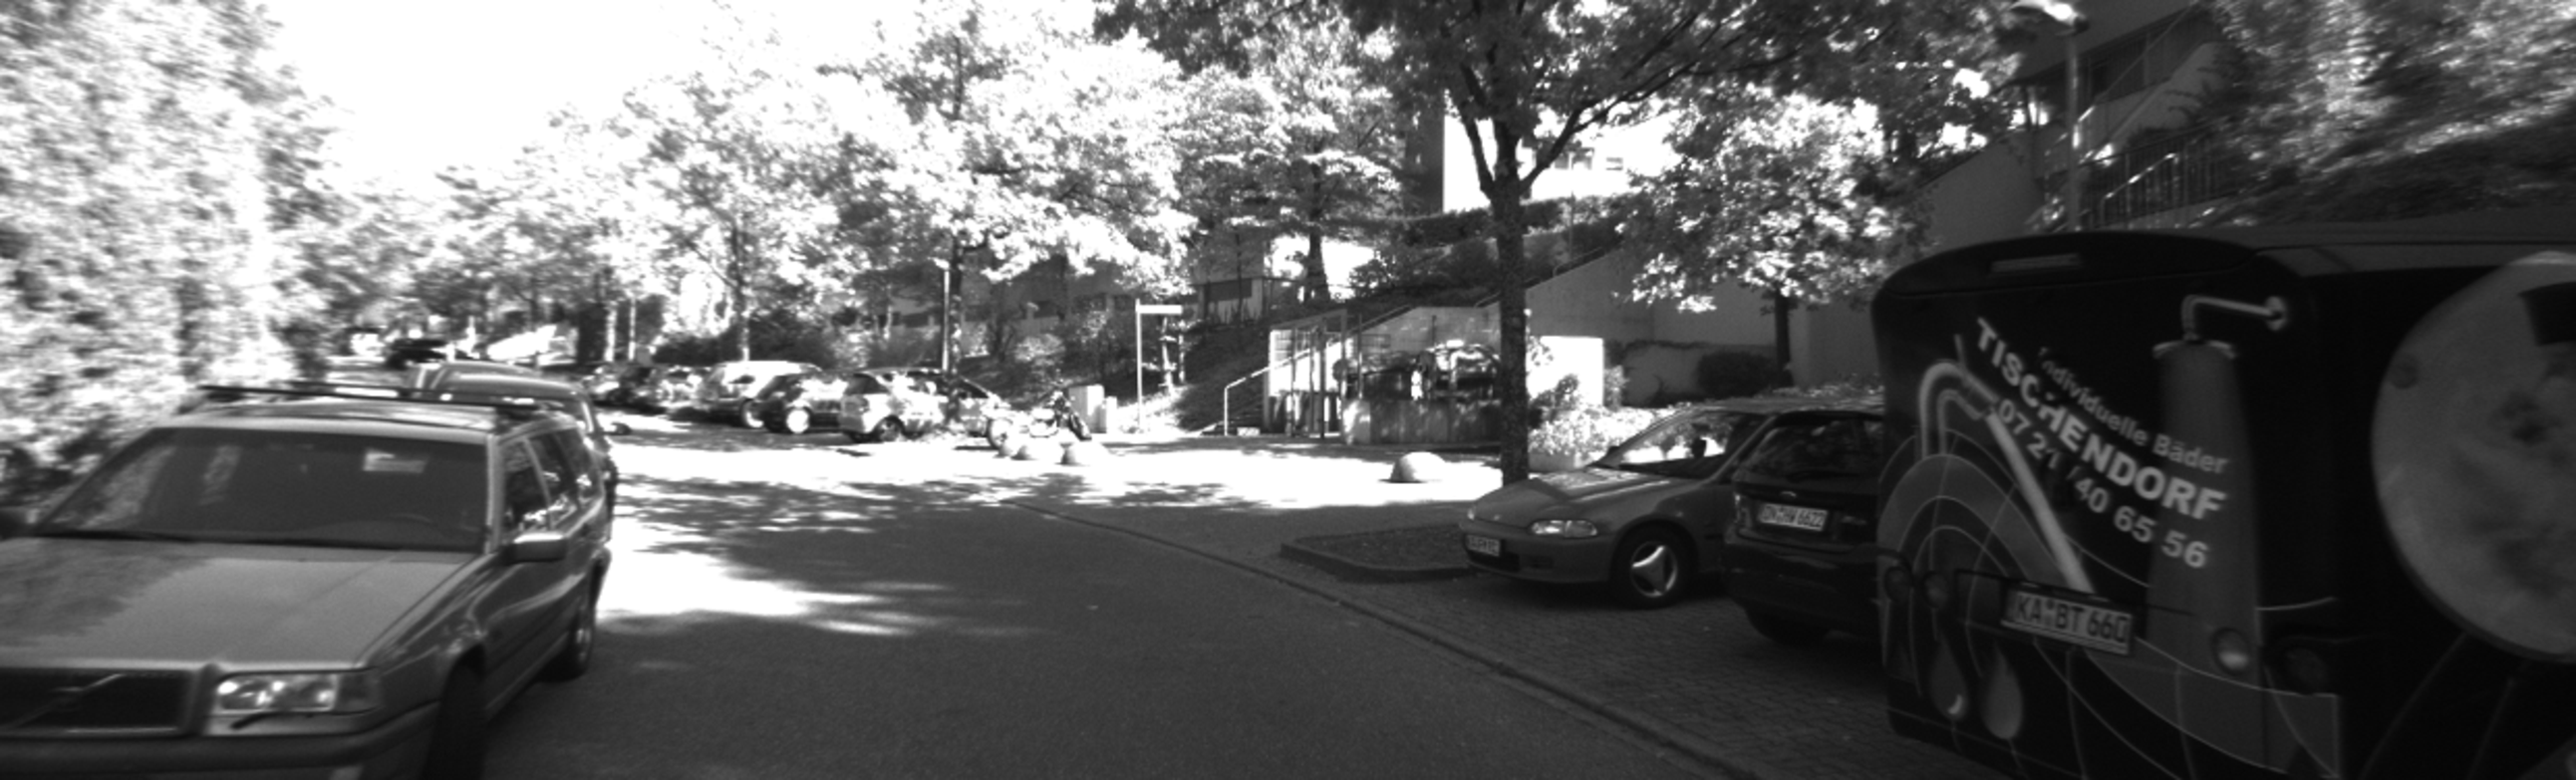
\includegraphics[height=1in]{KITTI02.pdf}}
    \quad
\subfloat[TUM VI \textit{room3}\label{fig:room3}]
        {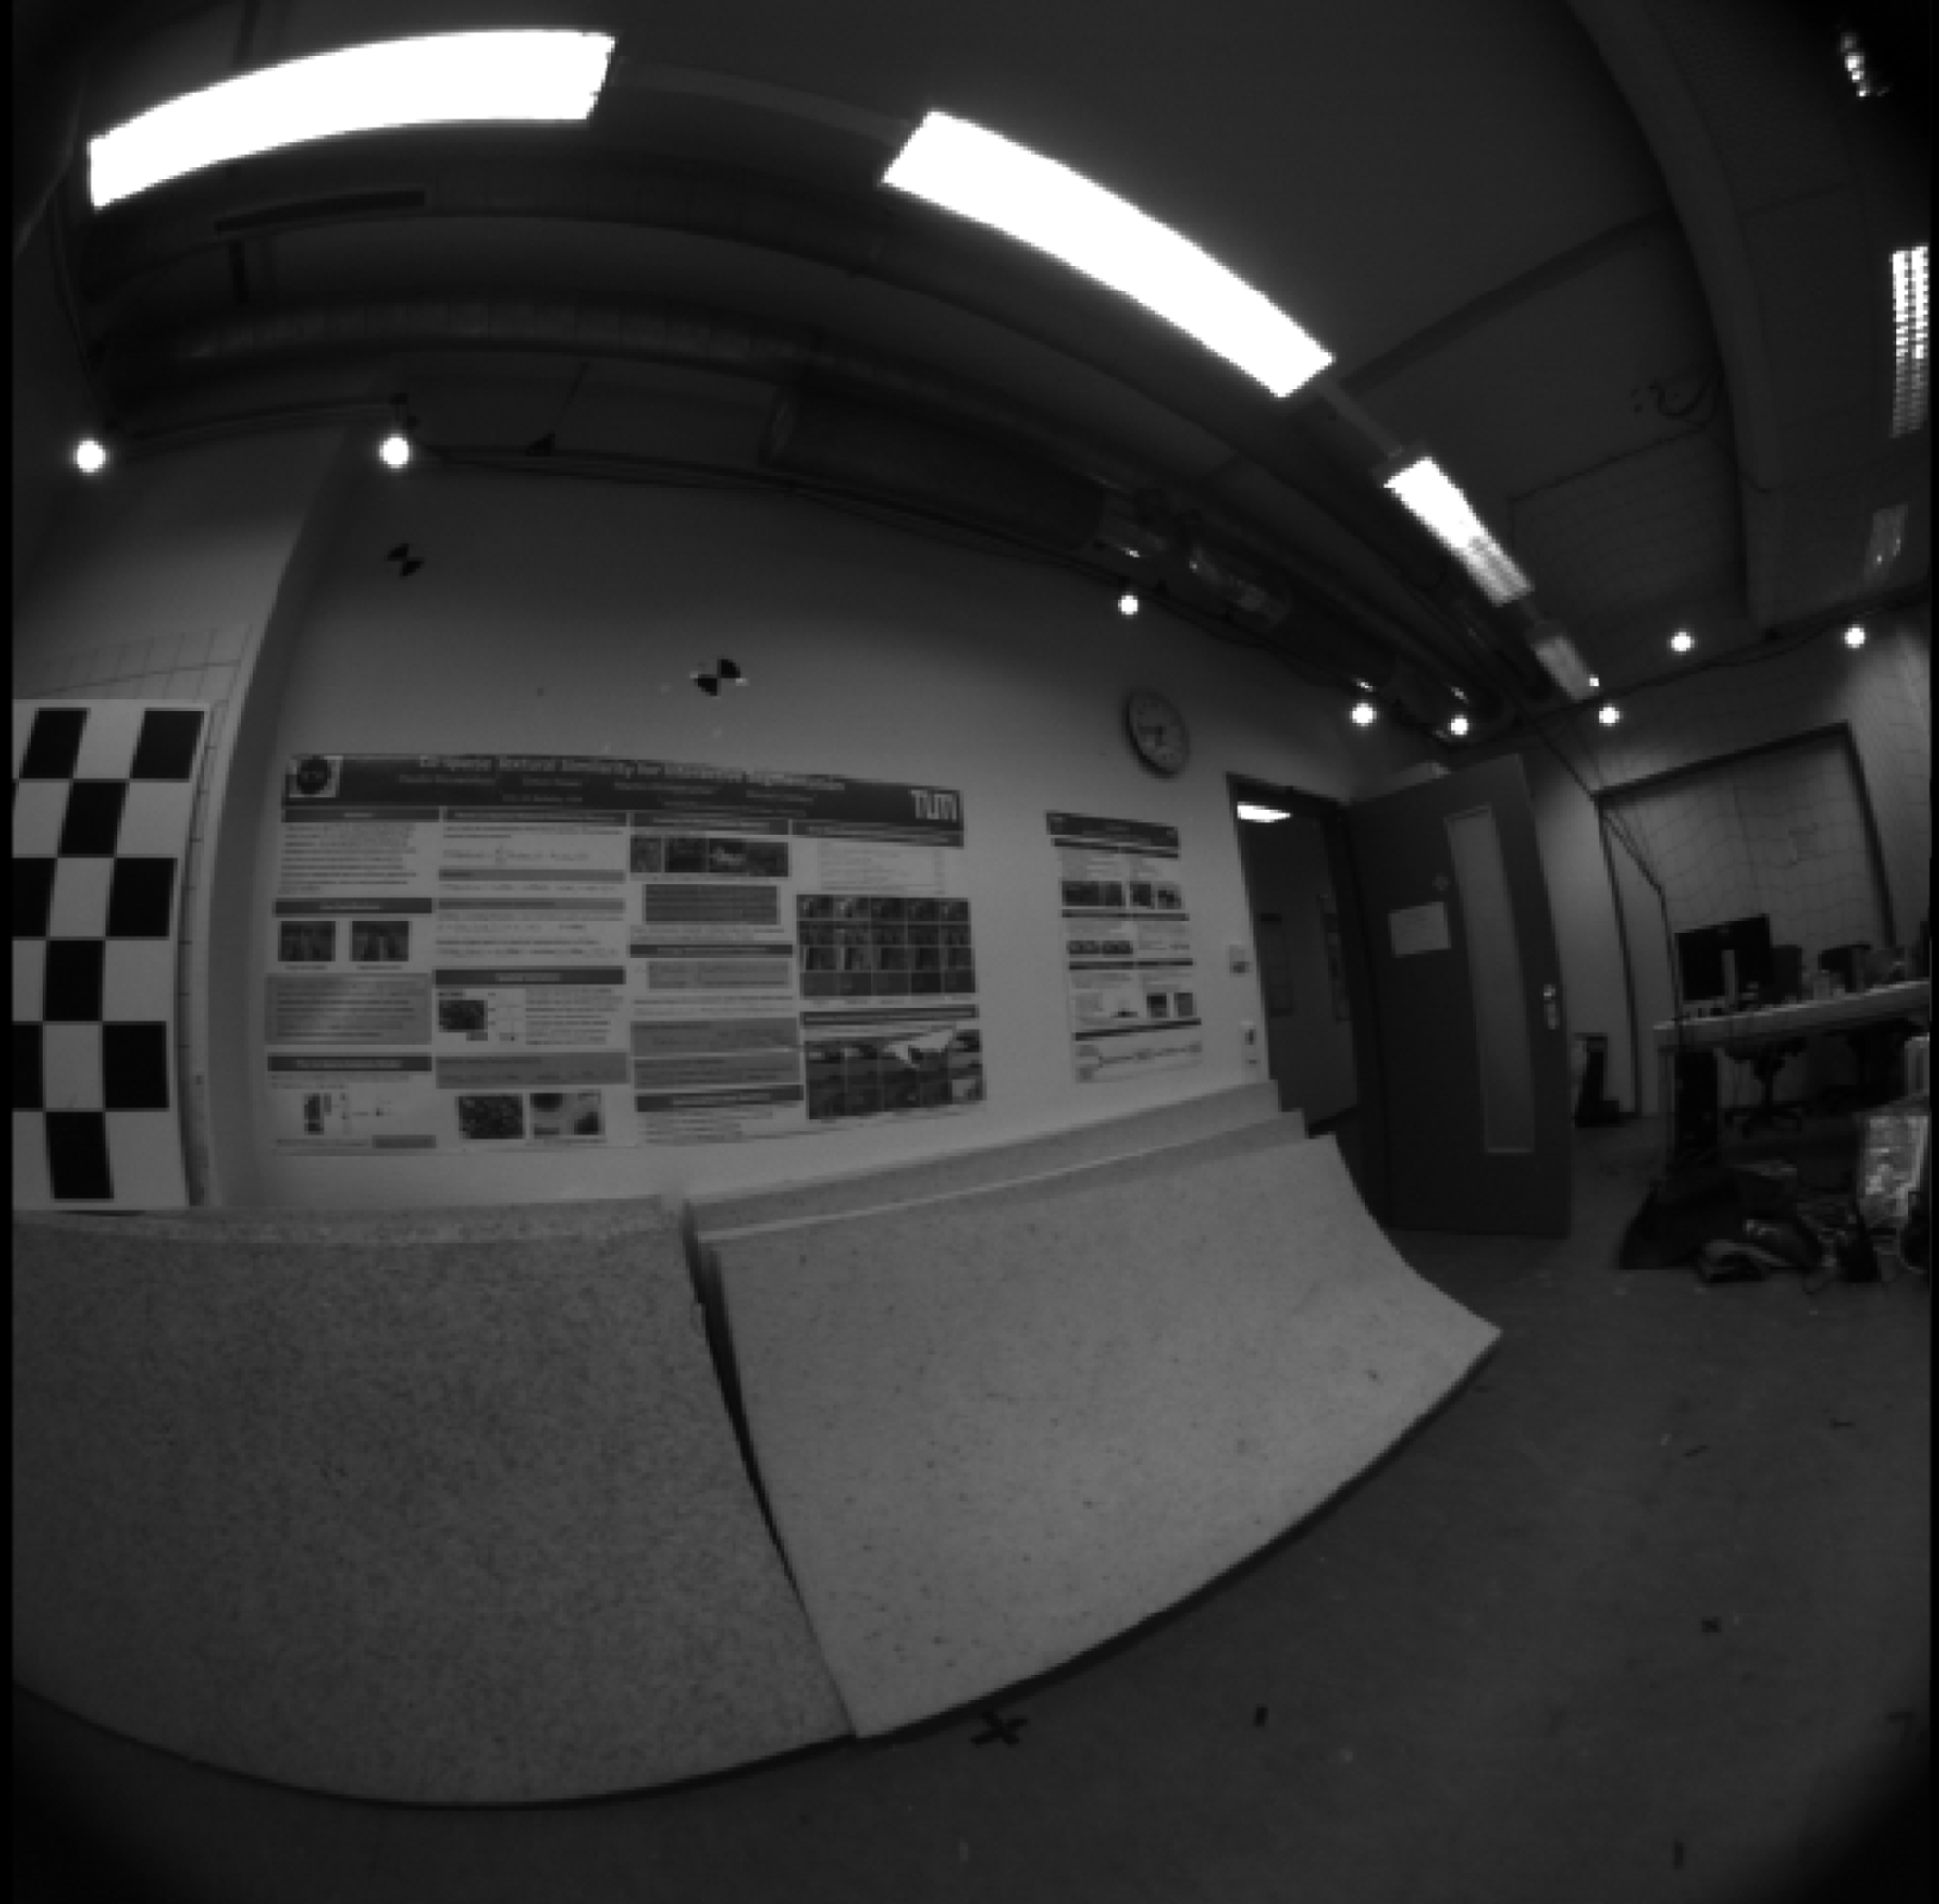
\includegraphics[height=1in]{TUM_VI_room.pdf}}
    \quad
\subfloat[TUM VI \textit{outdoor4}\label{fig:outdoor4}]
        {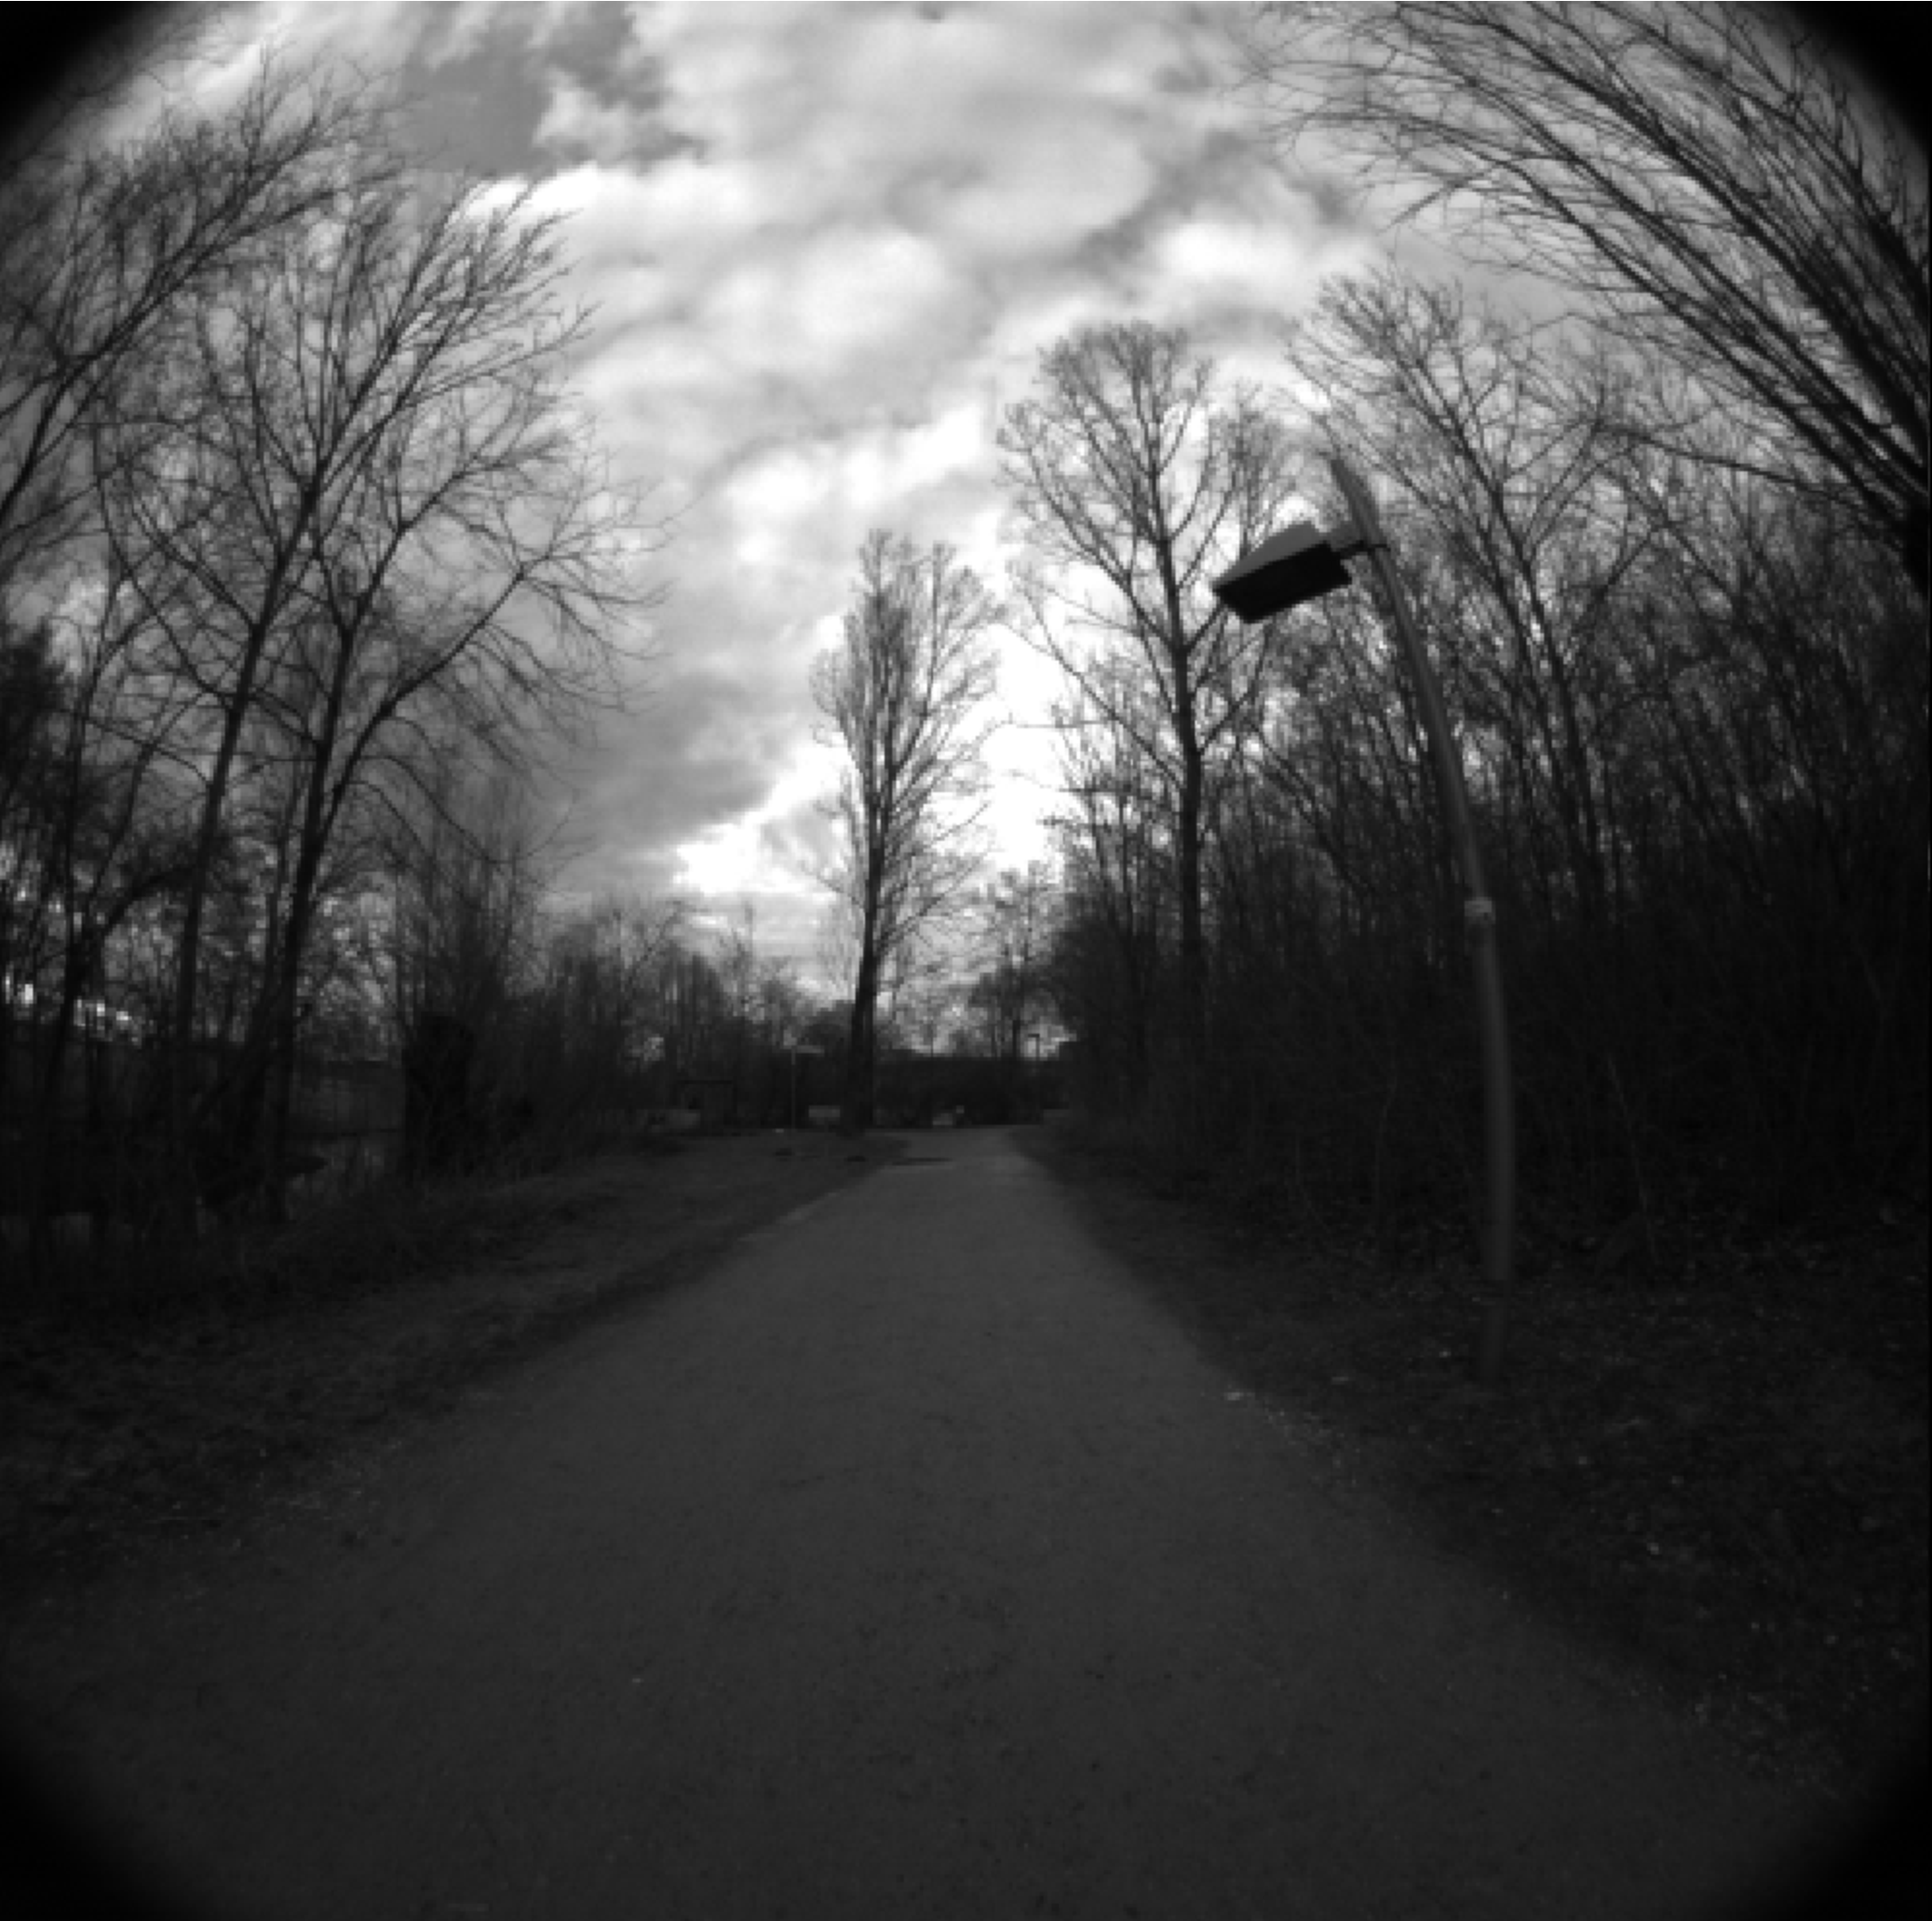
\includegraphics[height=1in]{TUM_VI_outdoor.pdf}}
            \quad
\subfloat[\textit{Conf. Hall1} \label{fig:mean and std of net24}]
        {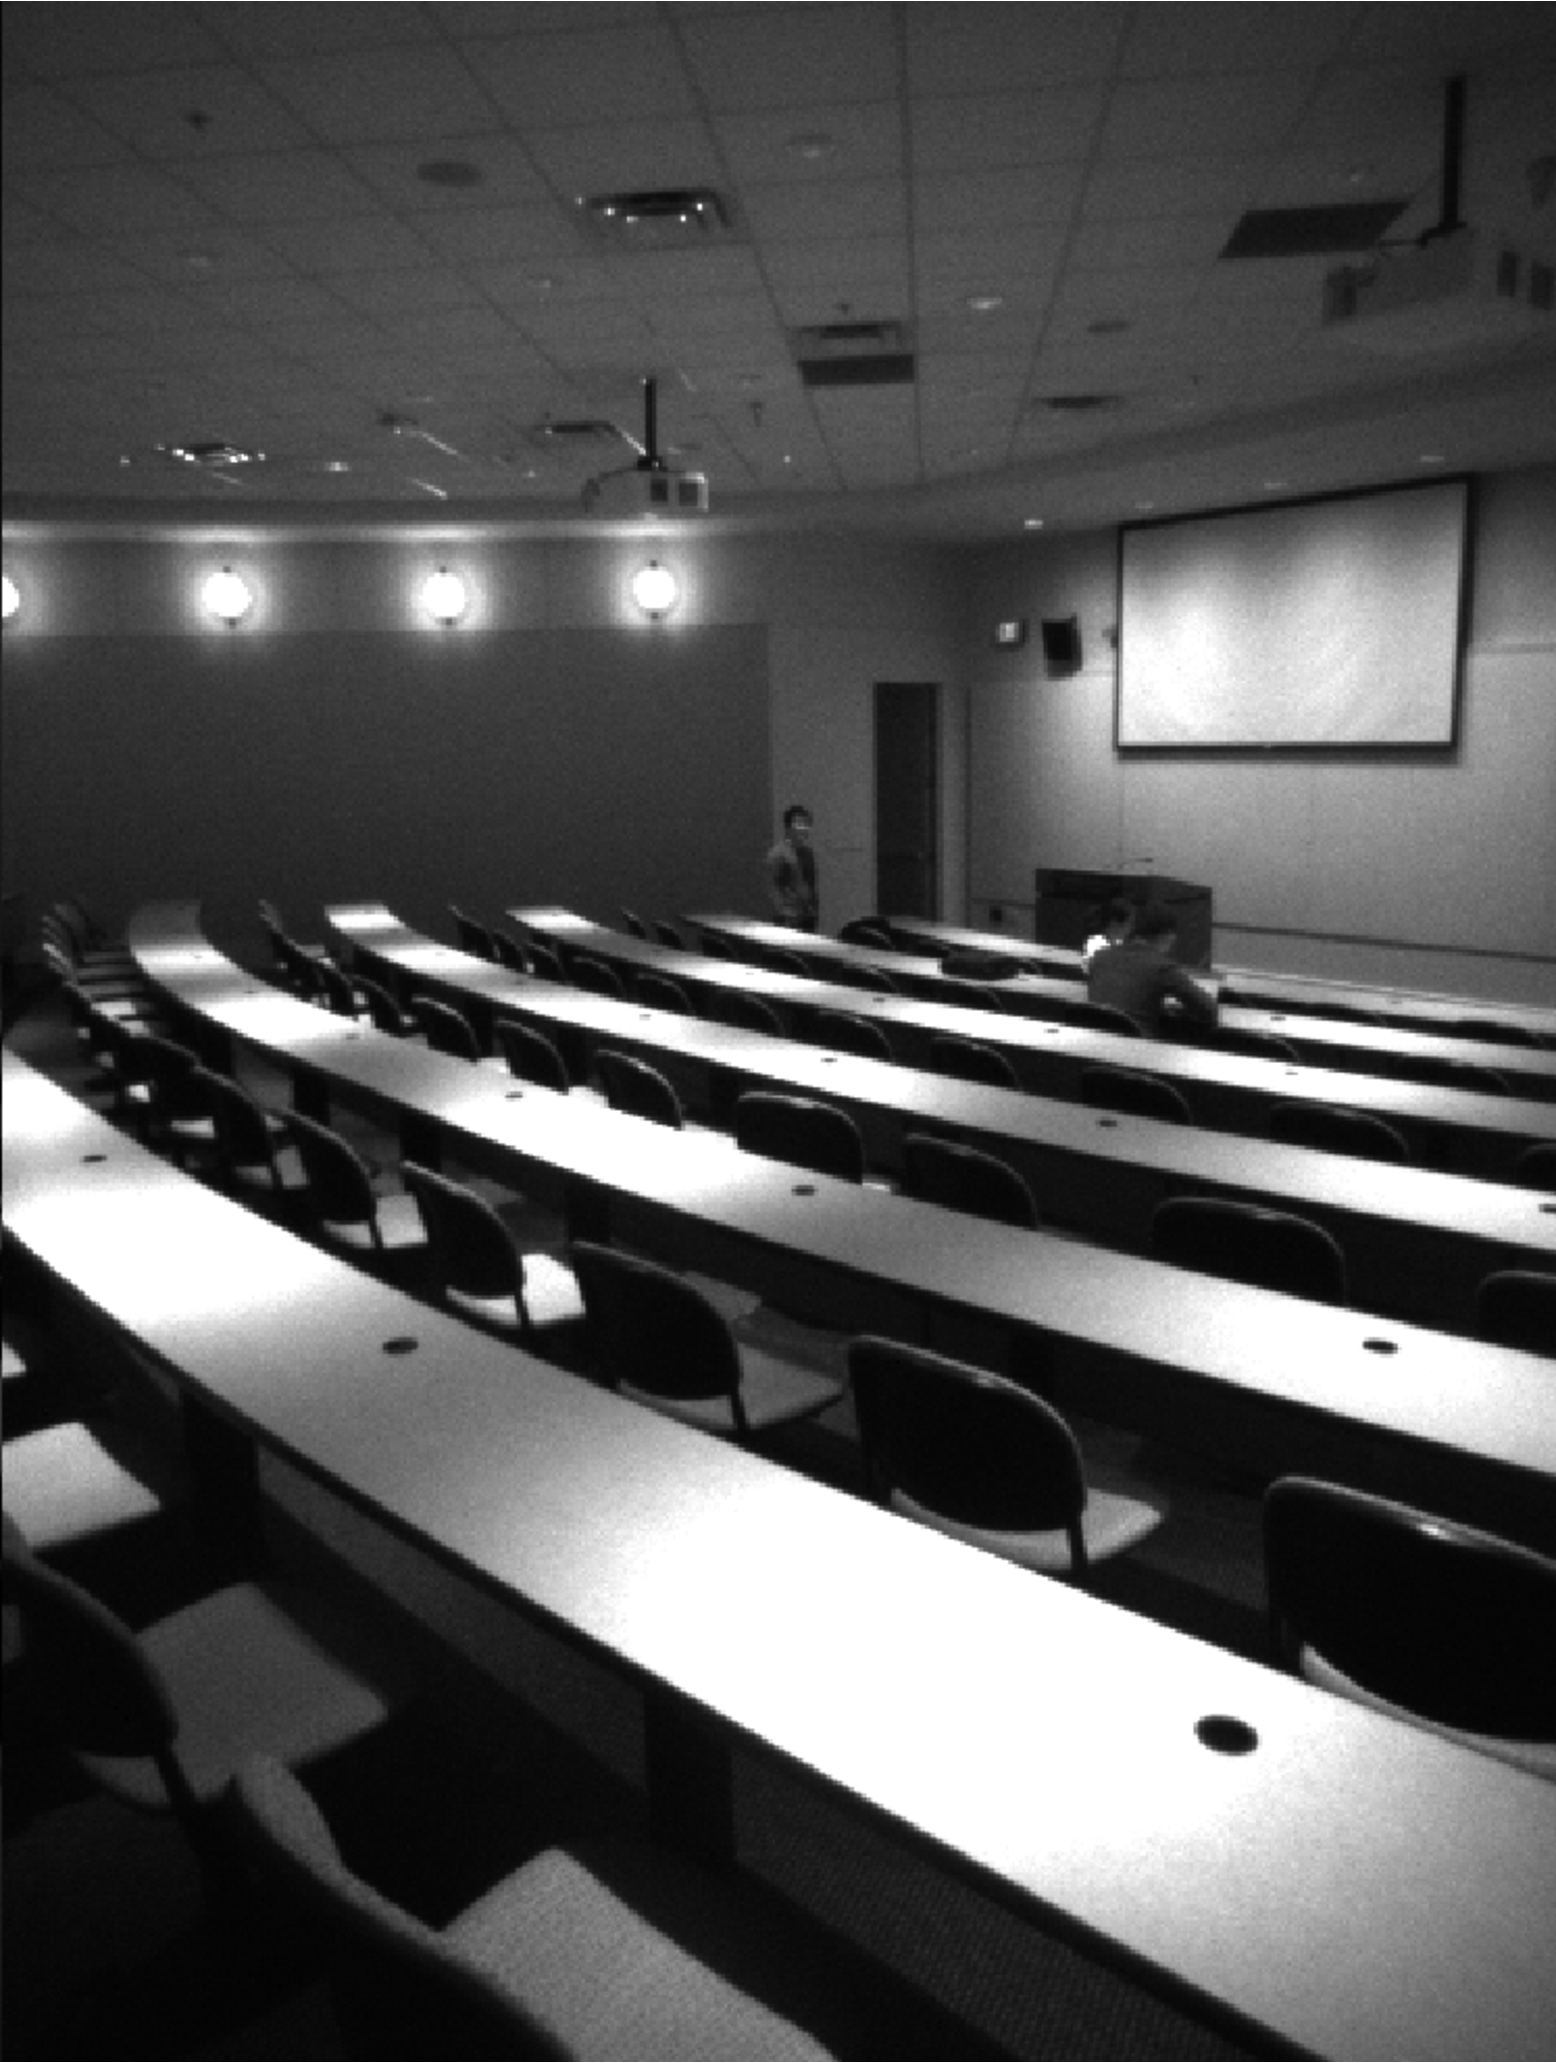
\includegraphics[height=1in]{Hololens.pdf}}
\\
\subfloat[KITTI \textit{Seq. 04}\label{fig:kitti04}]
        {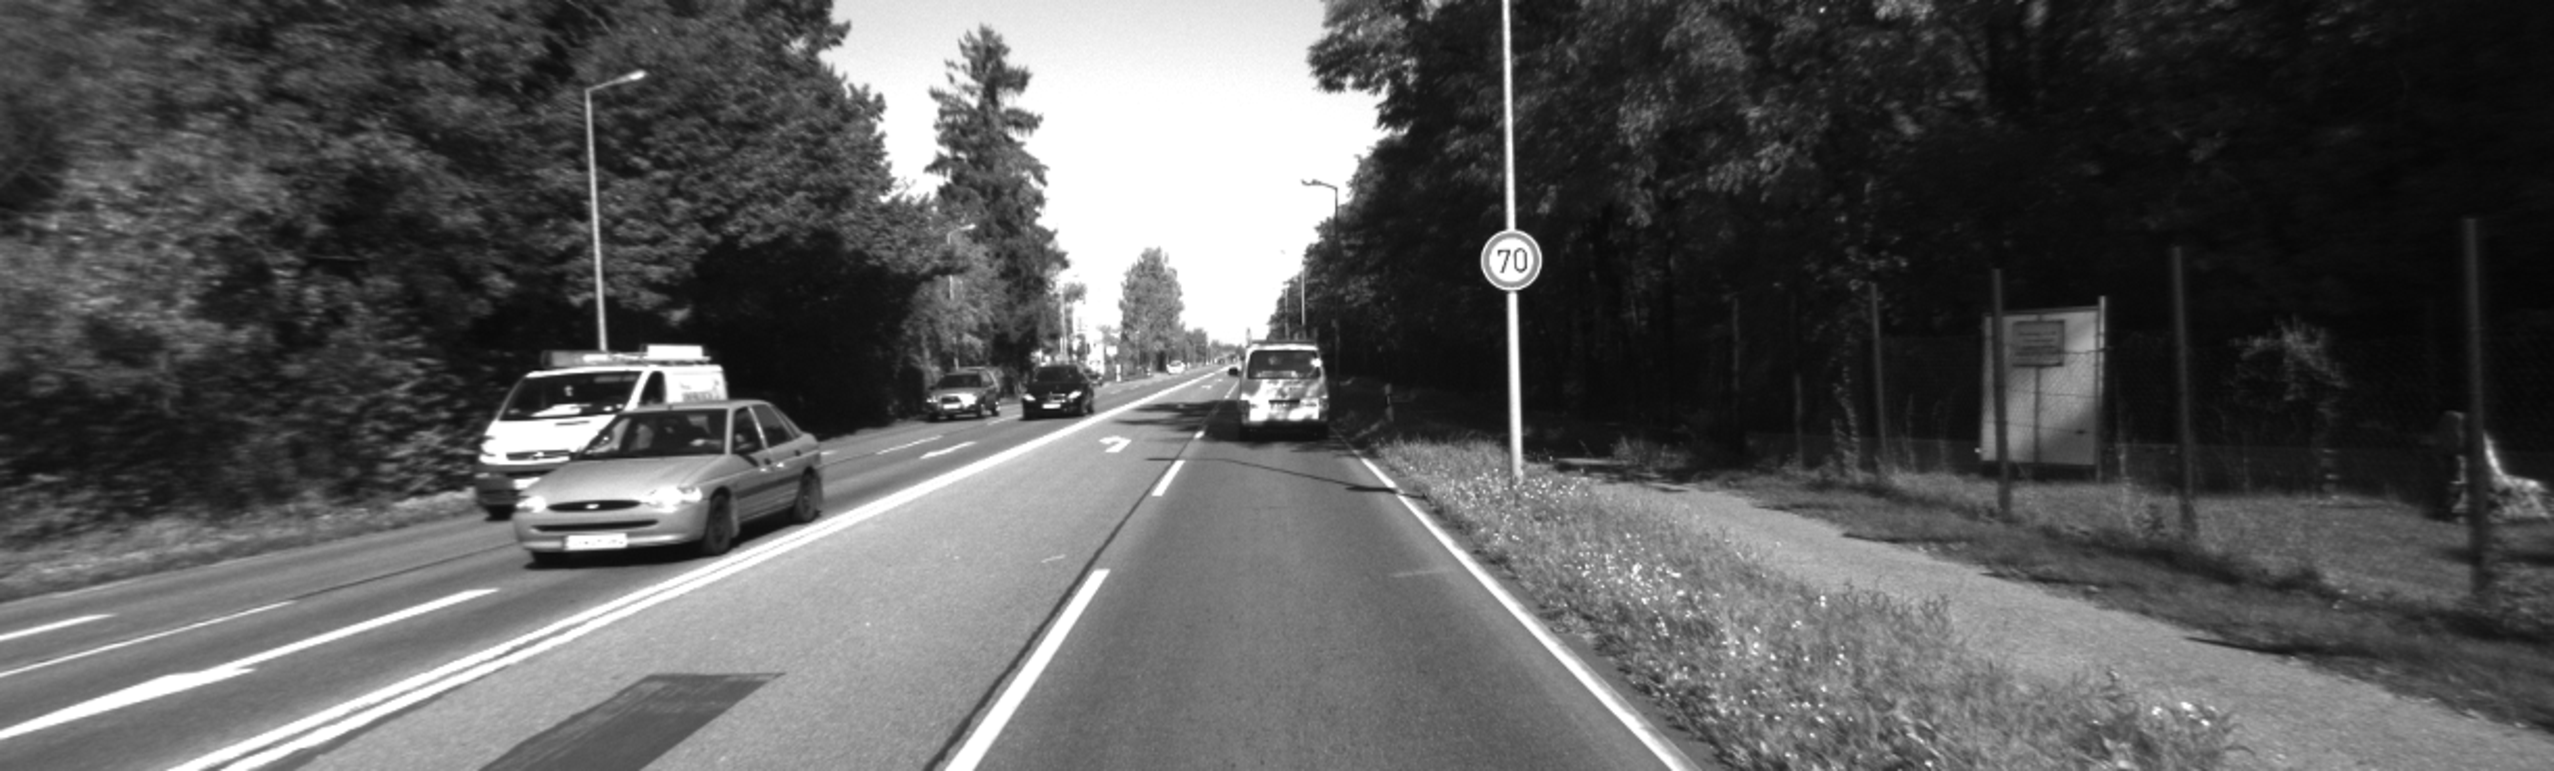
\includegraphics[height=1in]{KITTI04.pdf}}
    \quad
\subfloat[EuRoC \textit{MH 05 difficult}\label{fig:mh05}]
        {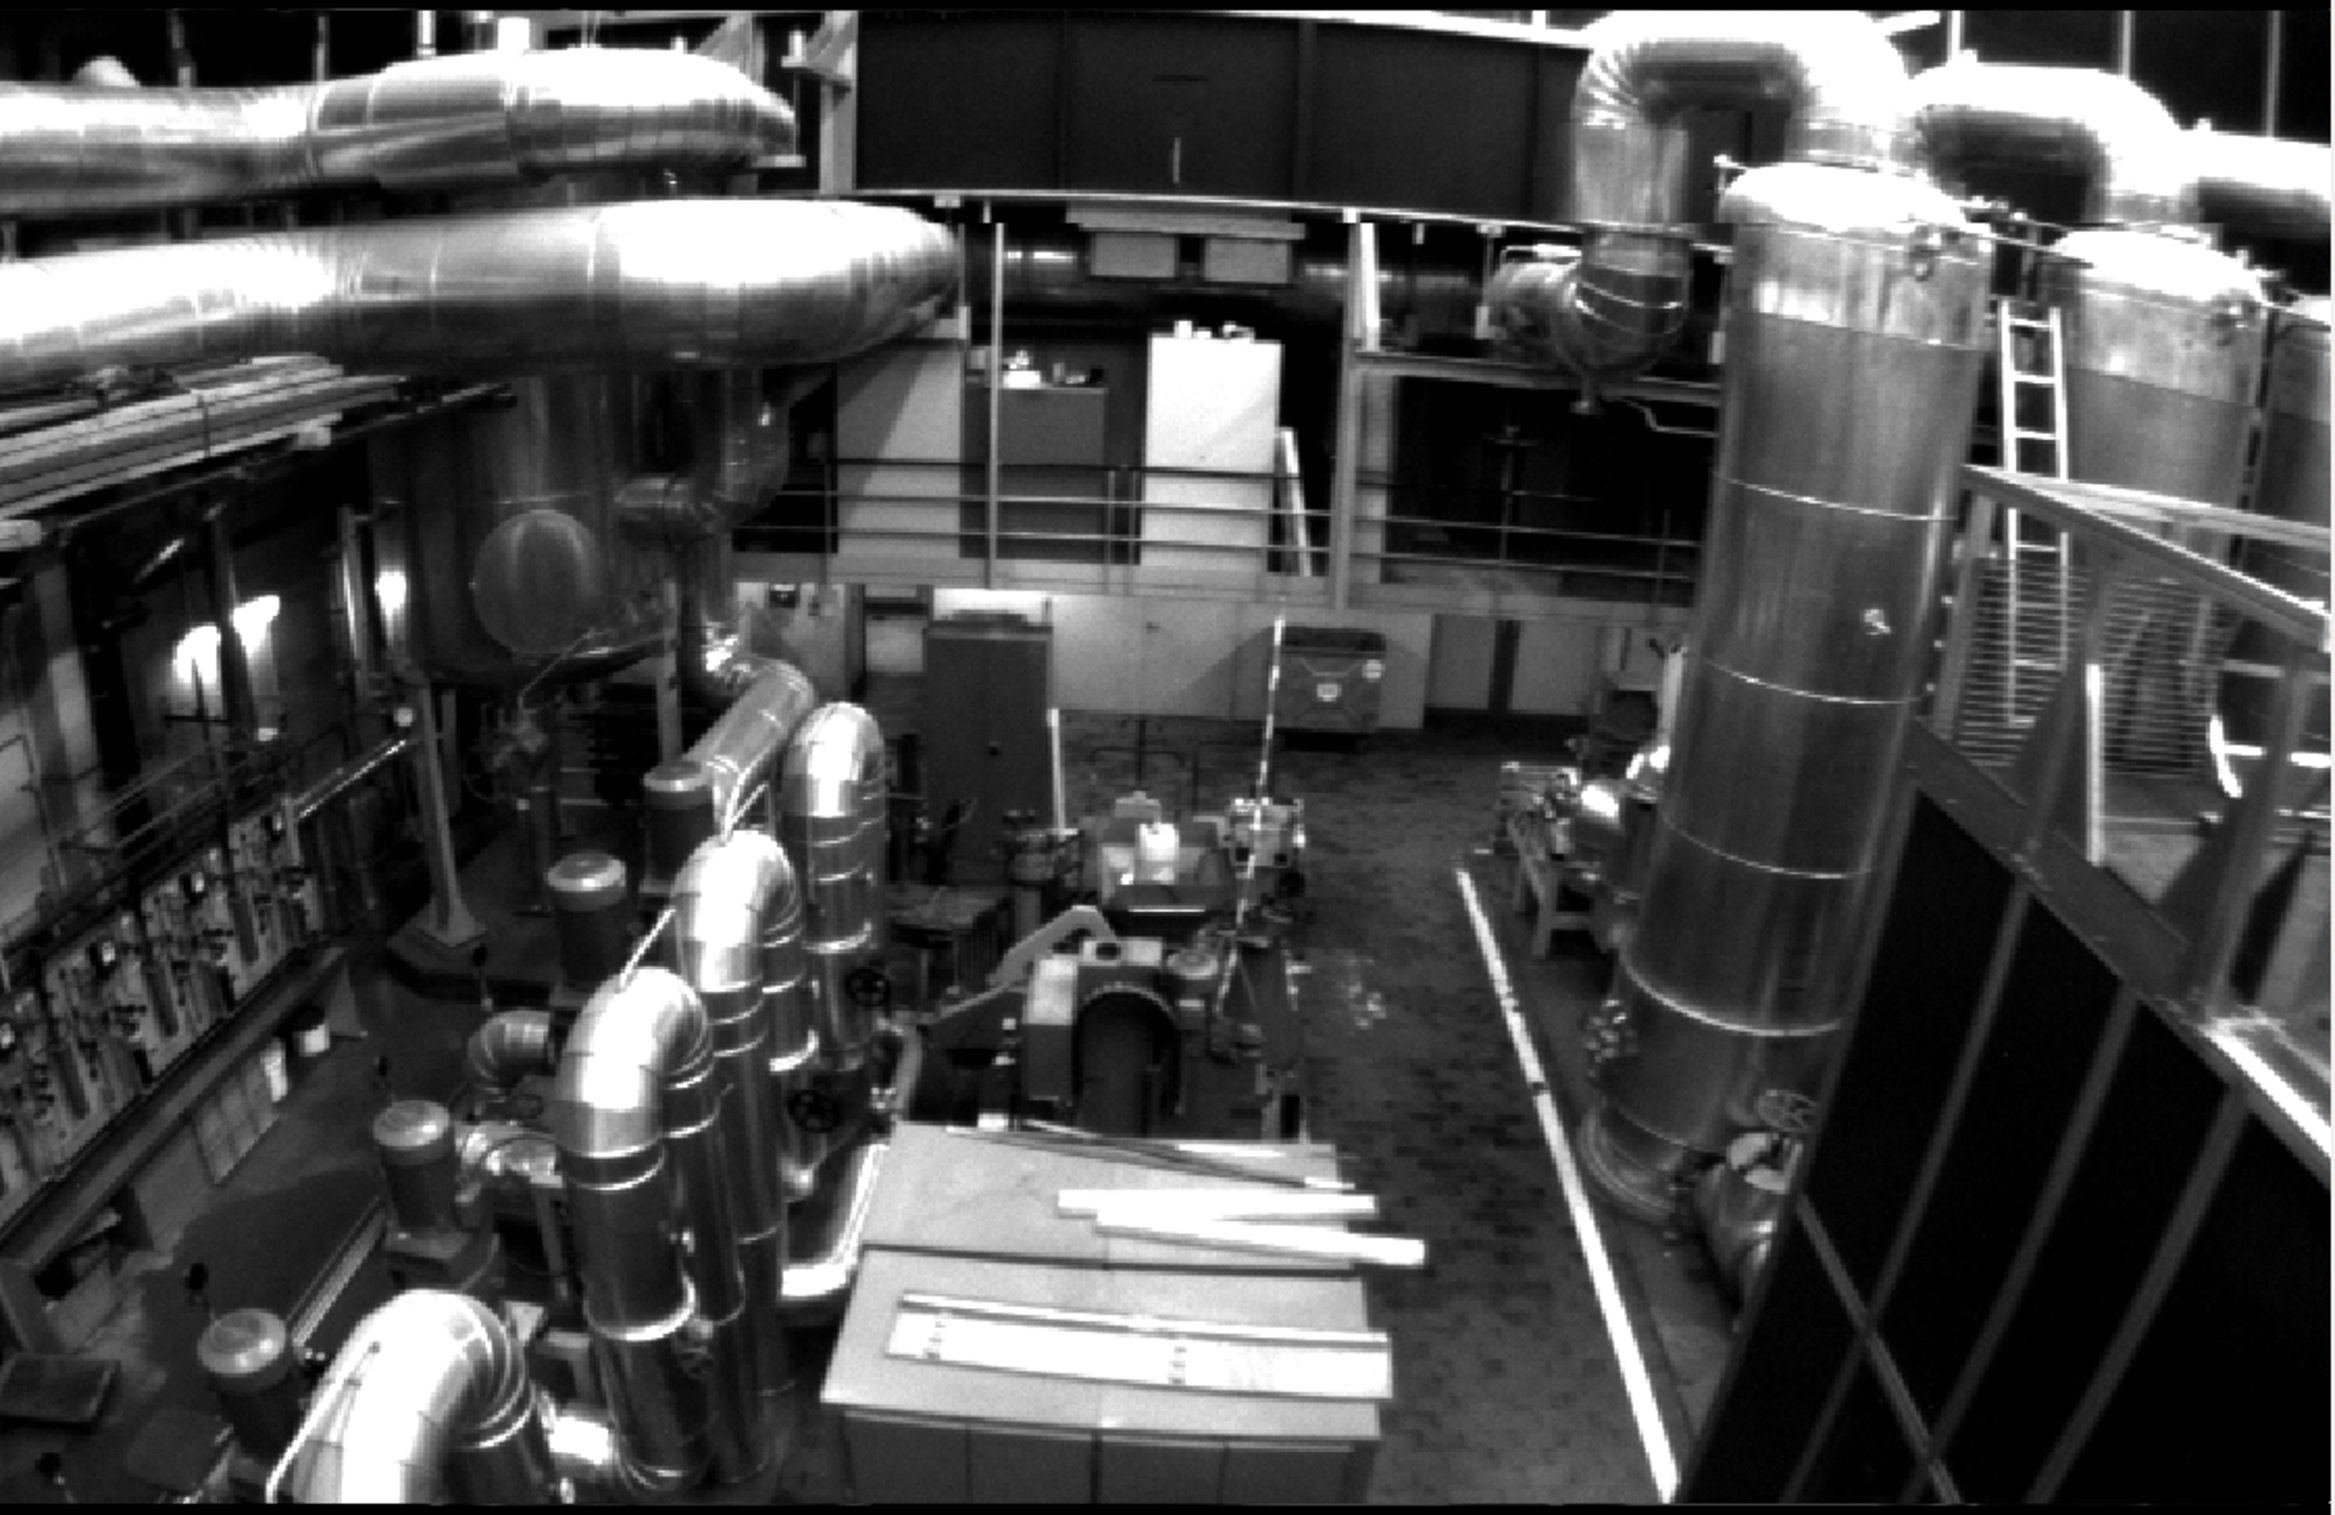
\includegraphics[height=1in]{MH05.pdf}}
    \quad
\subfloat[EuRoC \textit{V1 03 difficult}\label{fig:v103}]
        {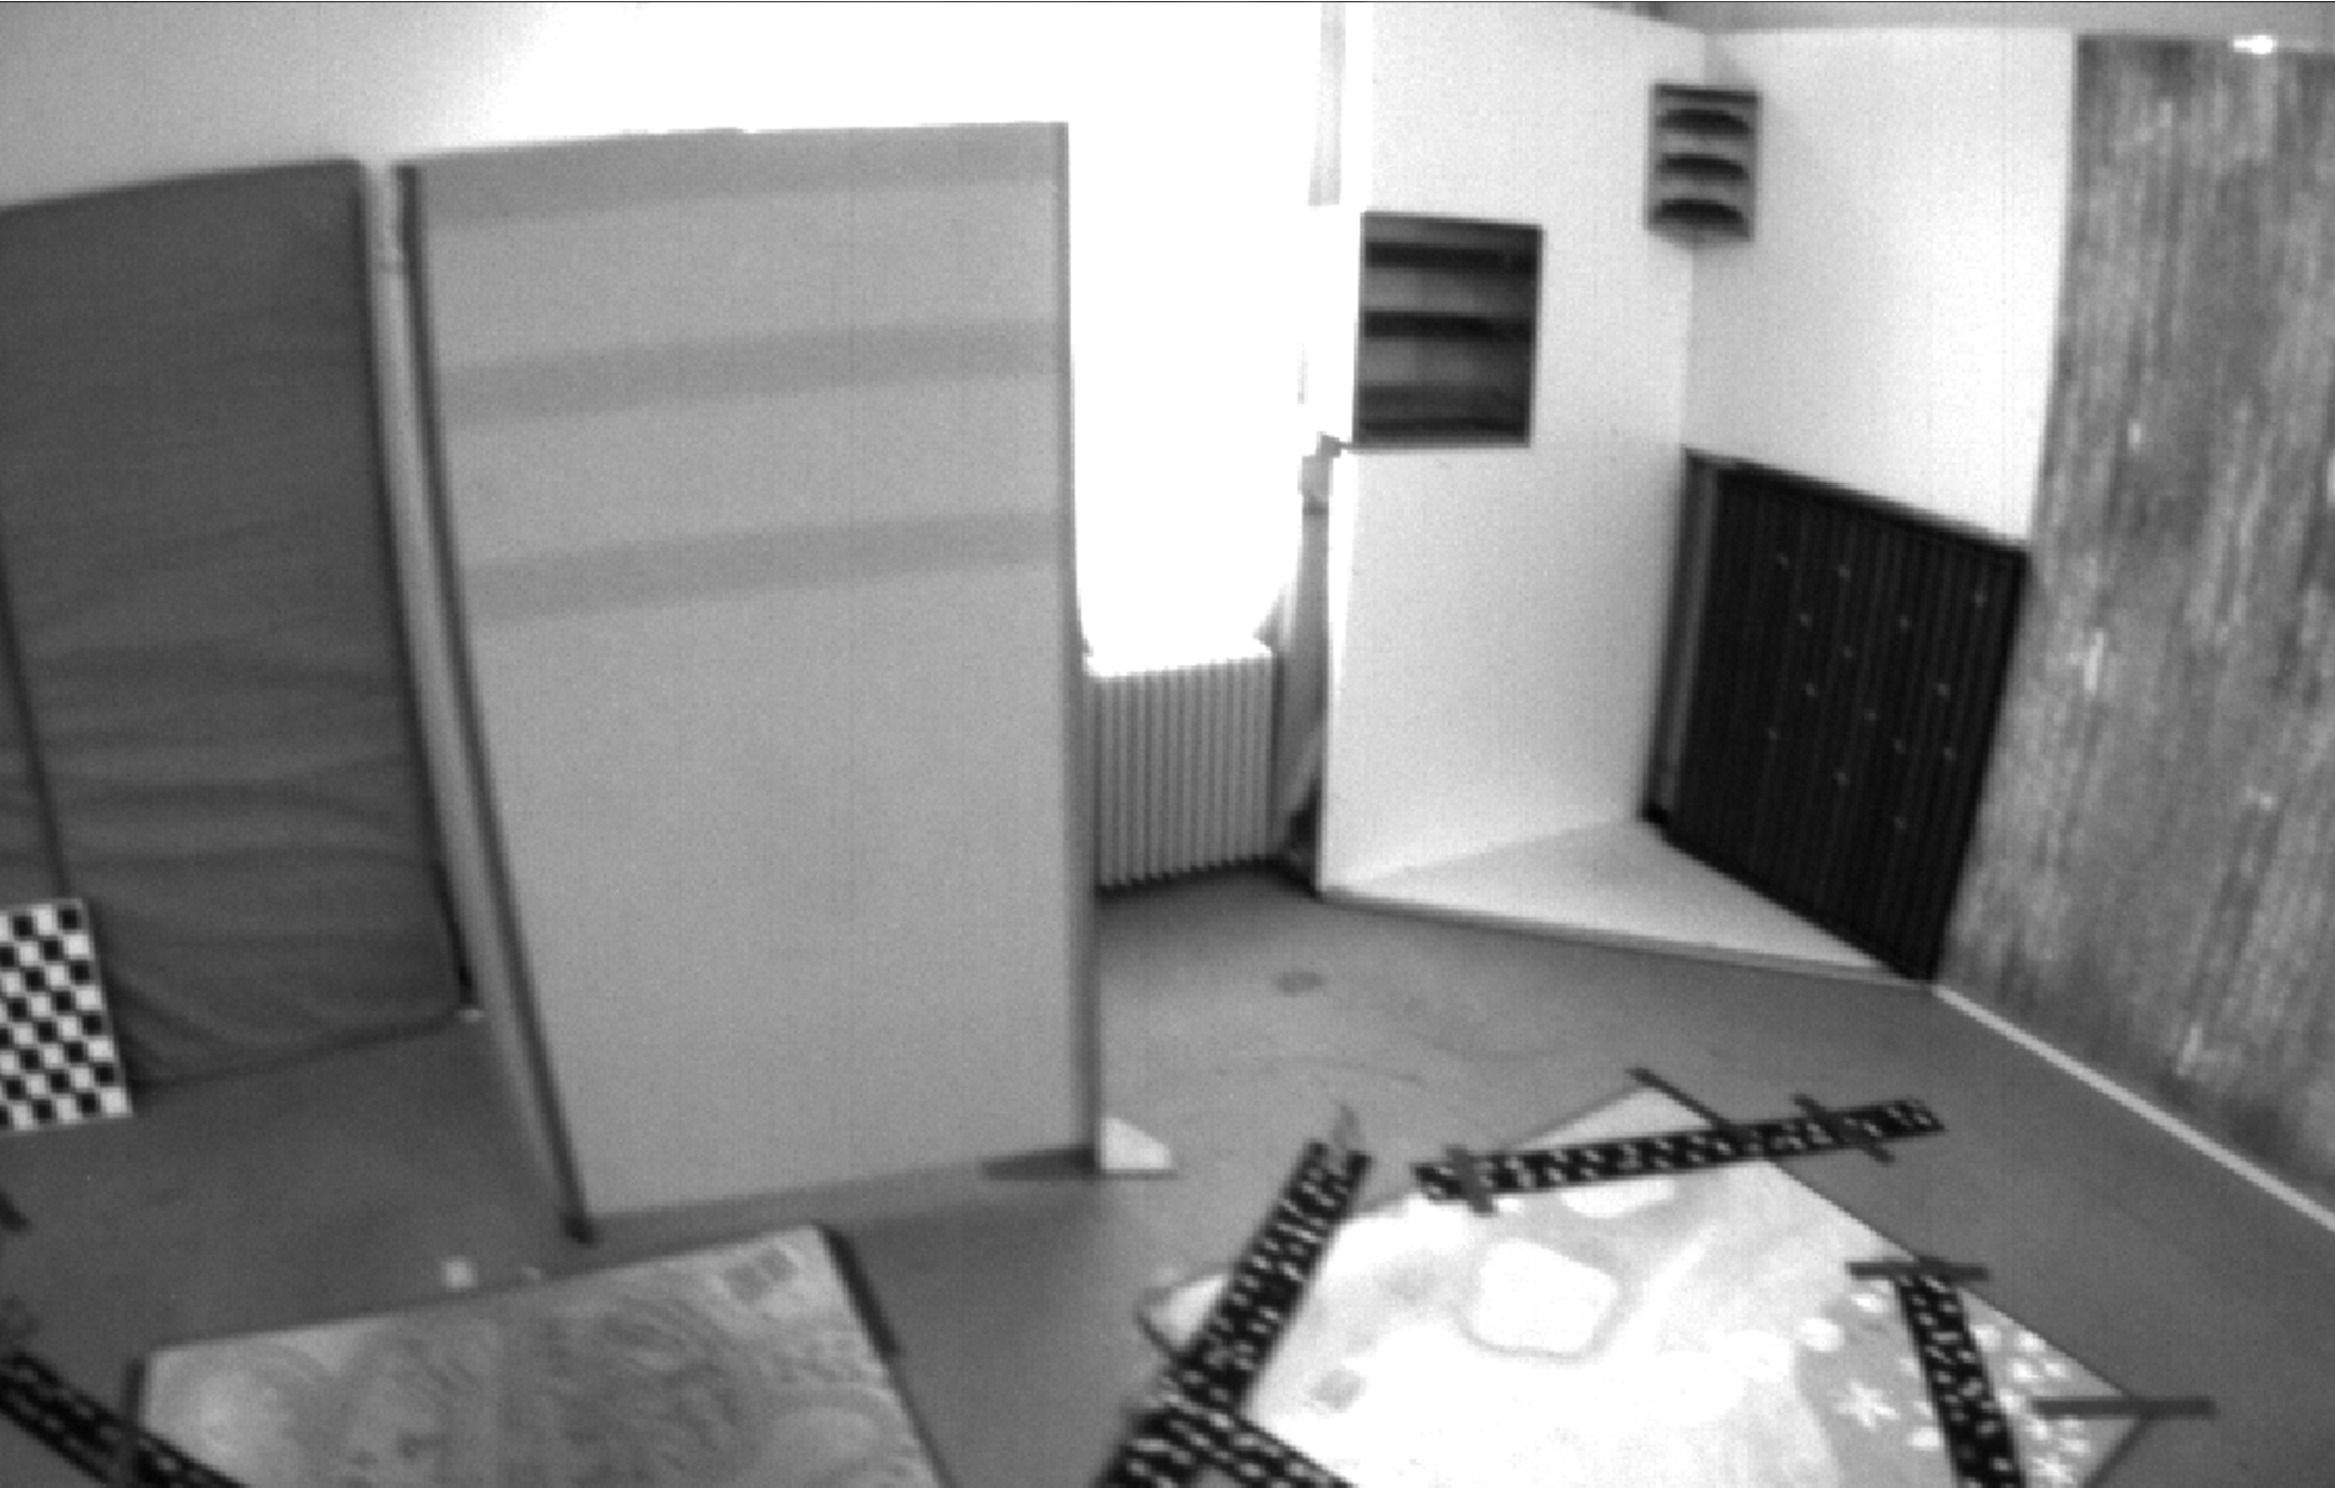
\includegraphics[height=1in]{V103.pdf}}
\\
\subfloat[NewCollege\label{fig:newcollege}]
        {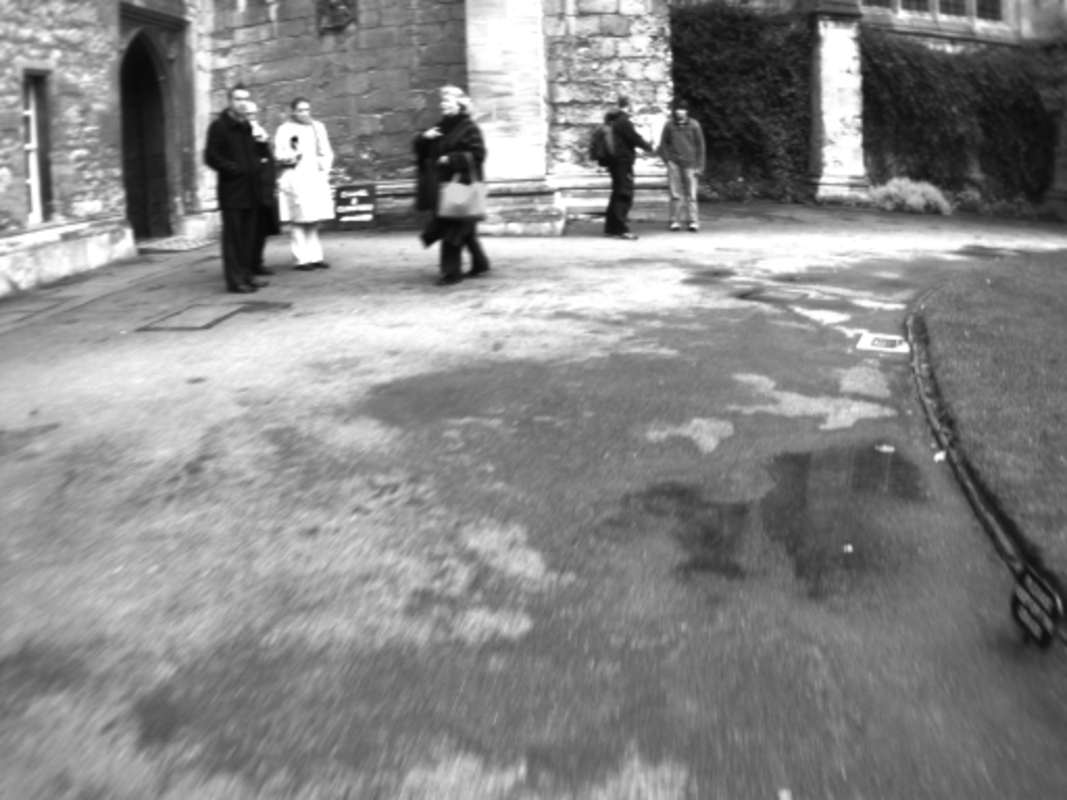
\includegraphics[height=1in]{NewCollege.pdf}}
    \quad
\subfloat[TUM RGBD \textit{desk person}\label{fig:deskperson}]
        {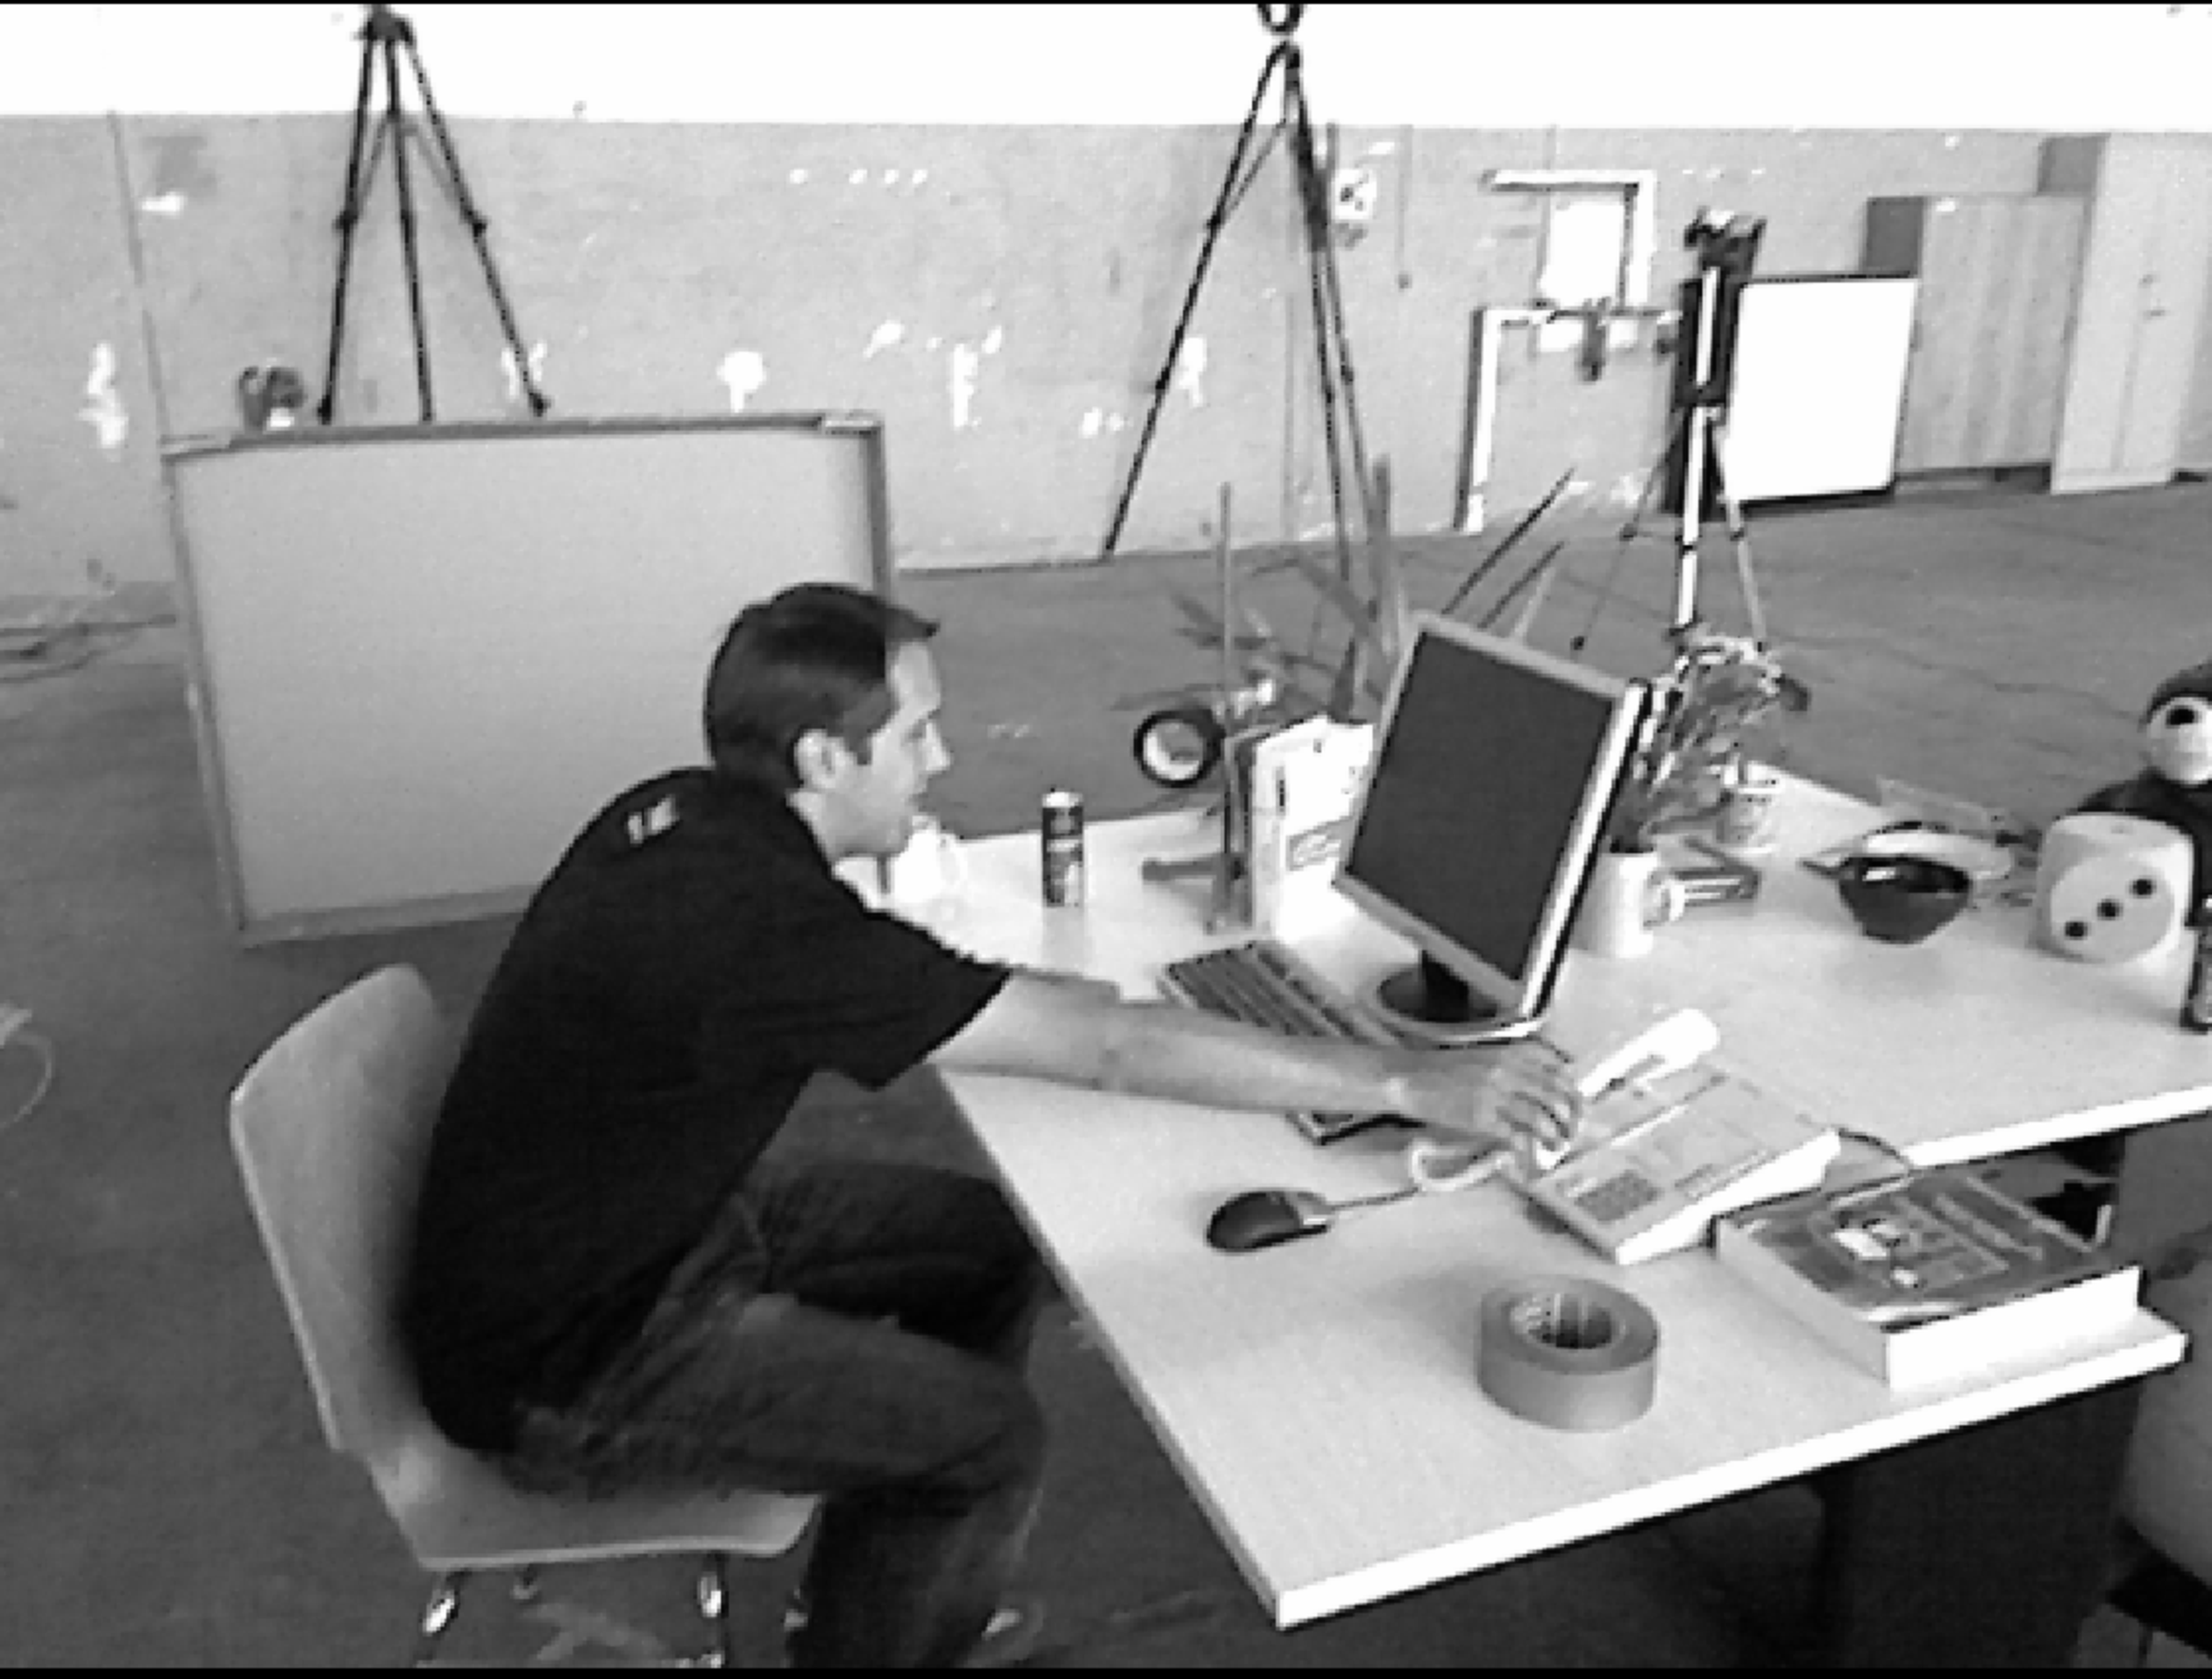
\includegraphics[height=1in]{TUM_RGBD.pdf}}
        \quad
\subfloat[\textit{Corridor} \label{fig:corridor}]
        {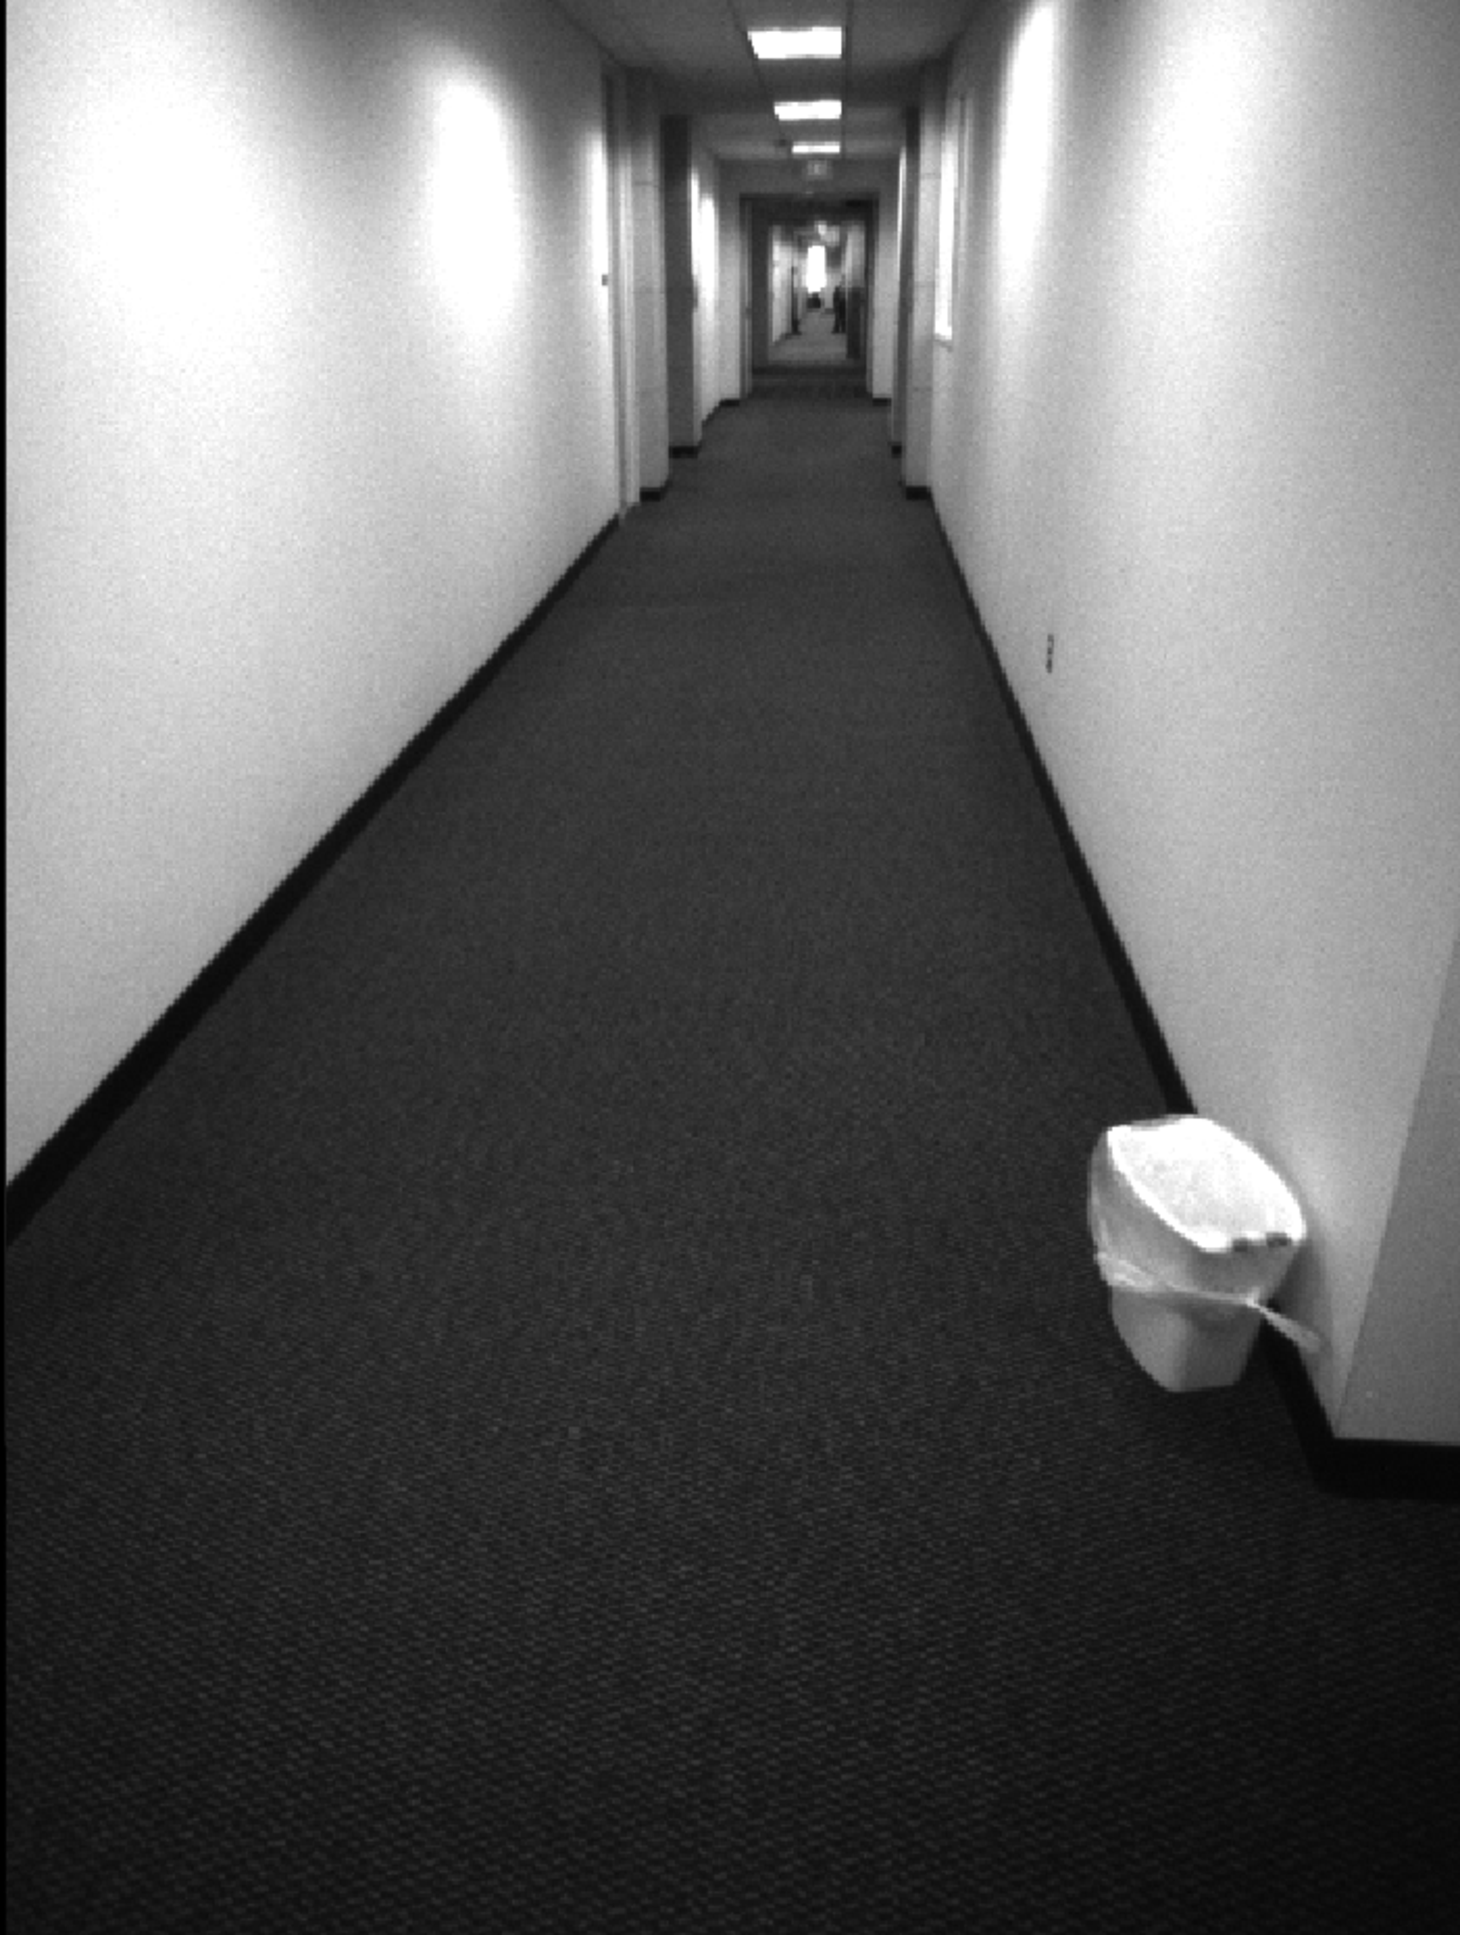
\includegraphics[height=1in]{corridor.pdf}}
        \quad
\subfloat[ICL NUIM \textit{lr kt0} \label{fig:lr00}]
        {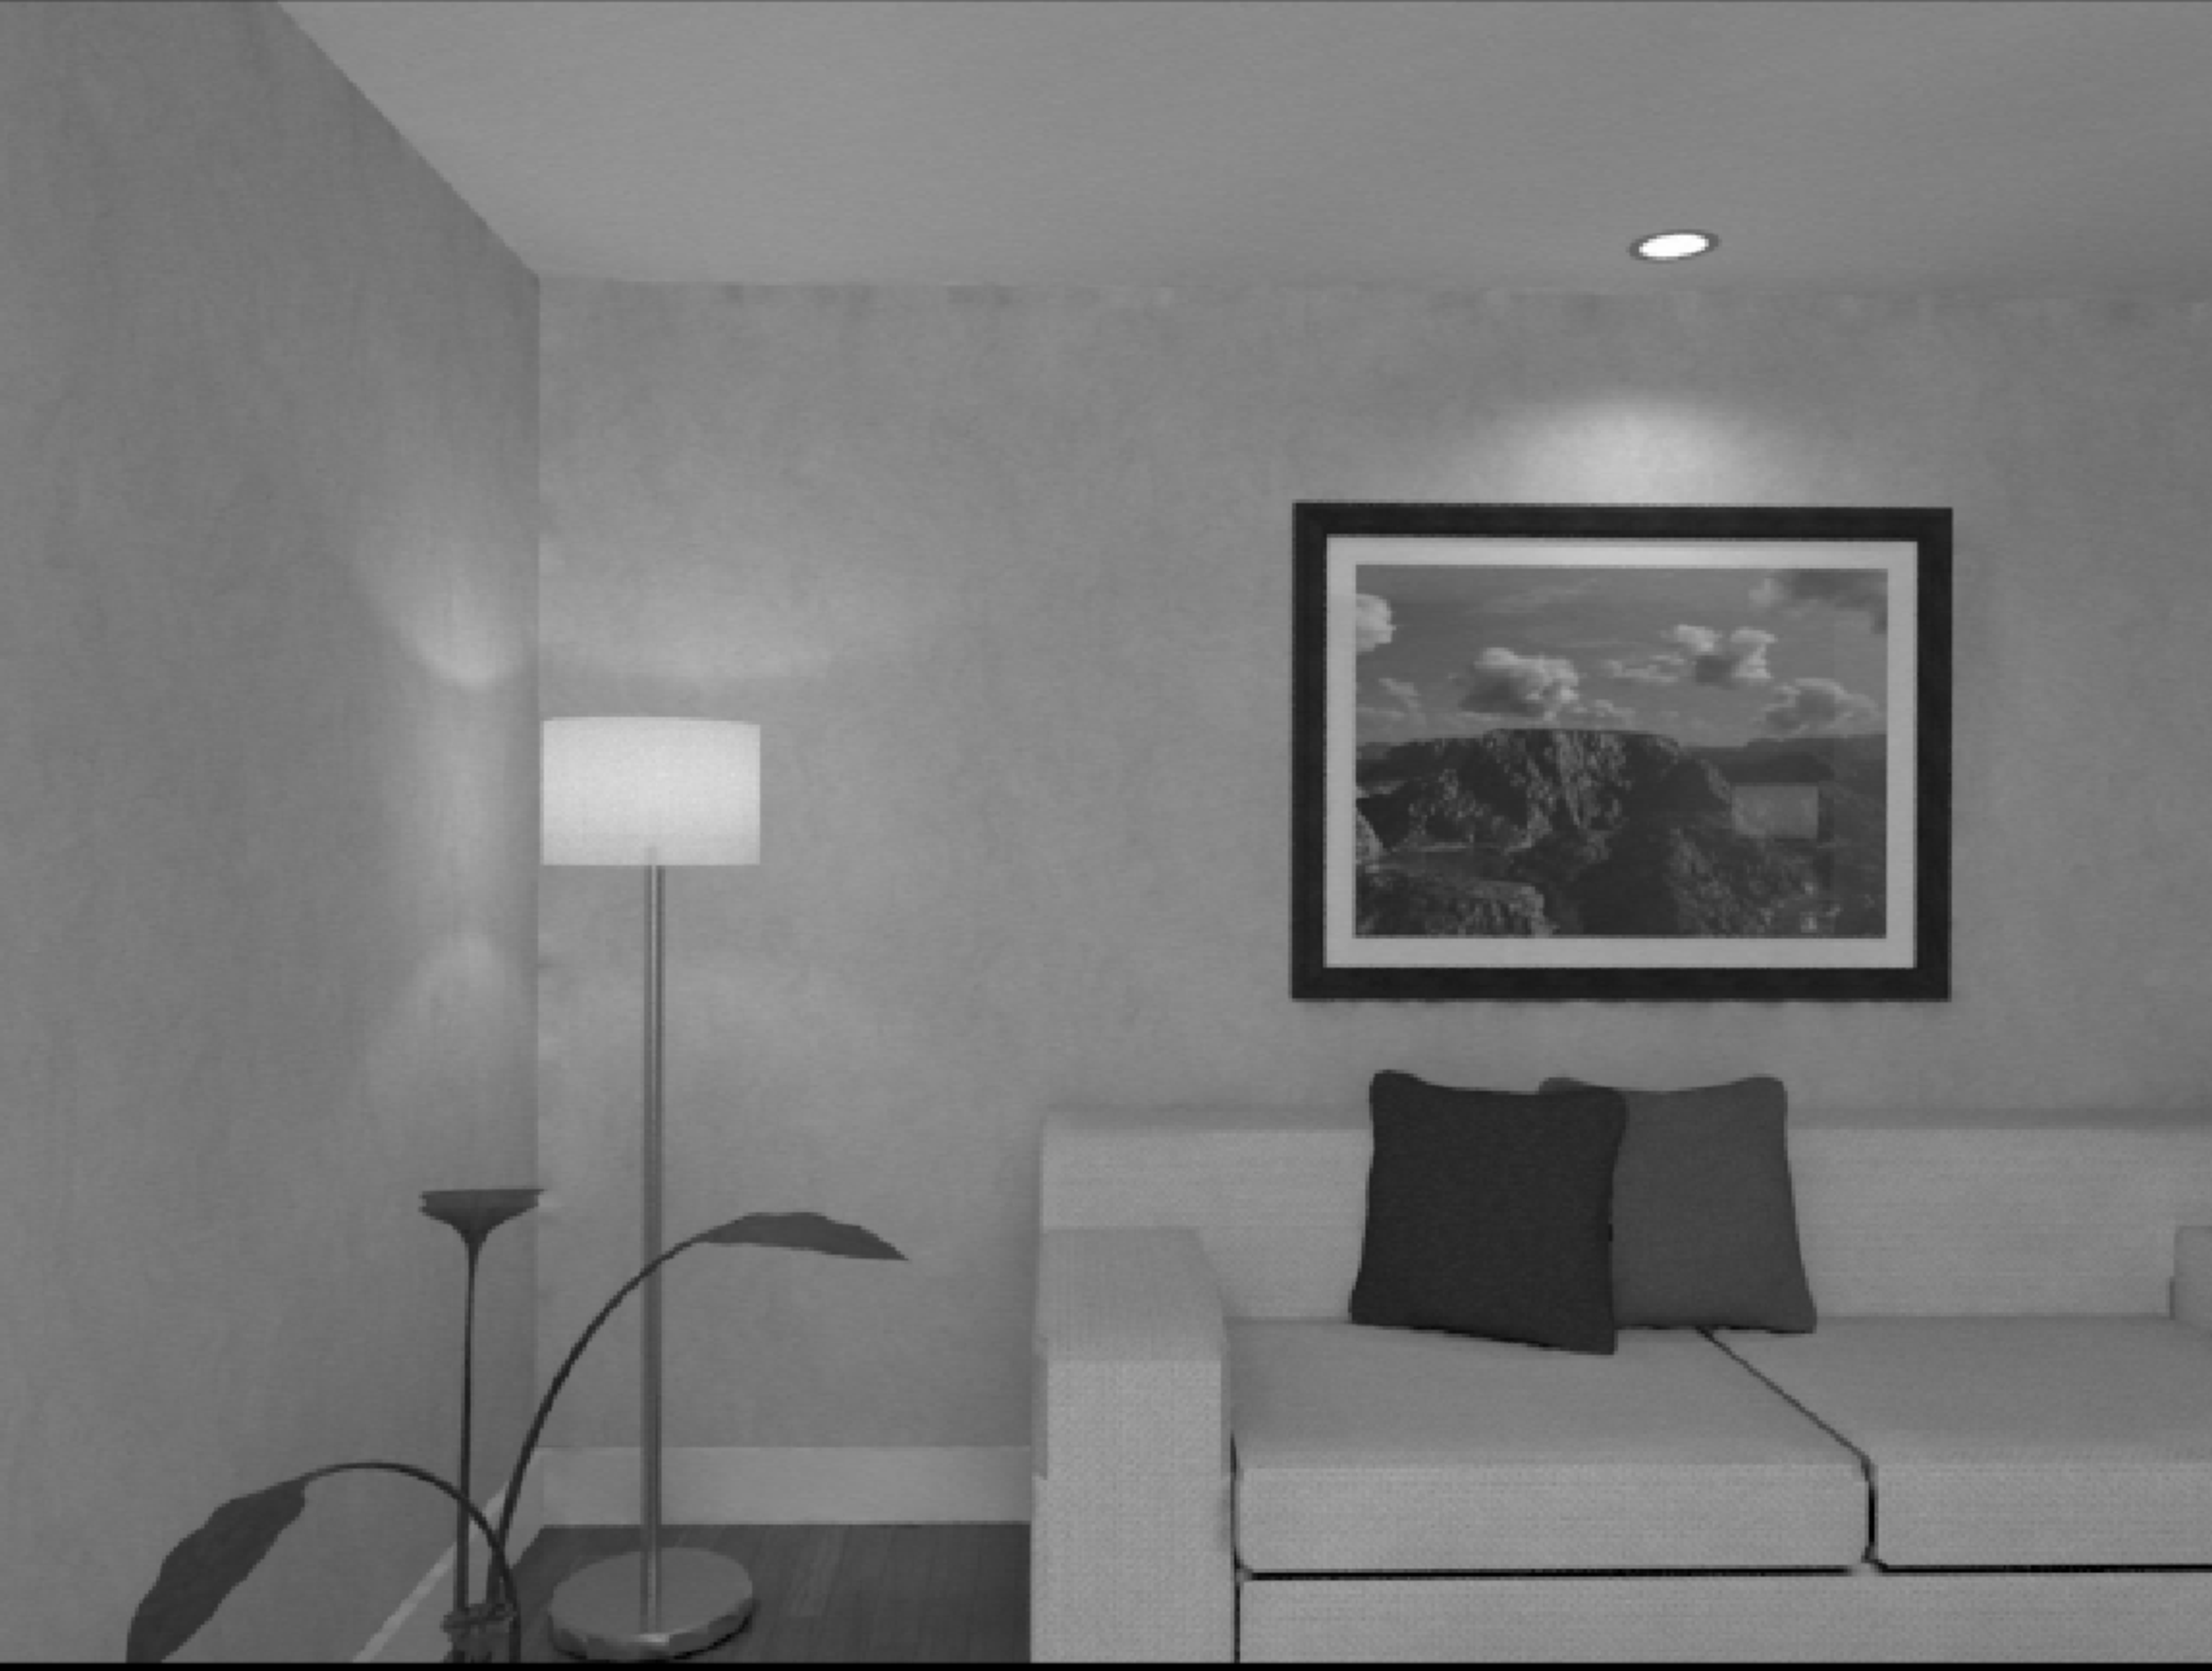
\includegraphics[height=1in]{lr00.pdf}}
                \quad
\subfloat[ICL NUIM \textit{of kt3} \label{fig:of03}]
        {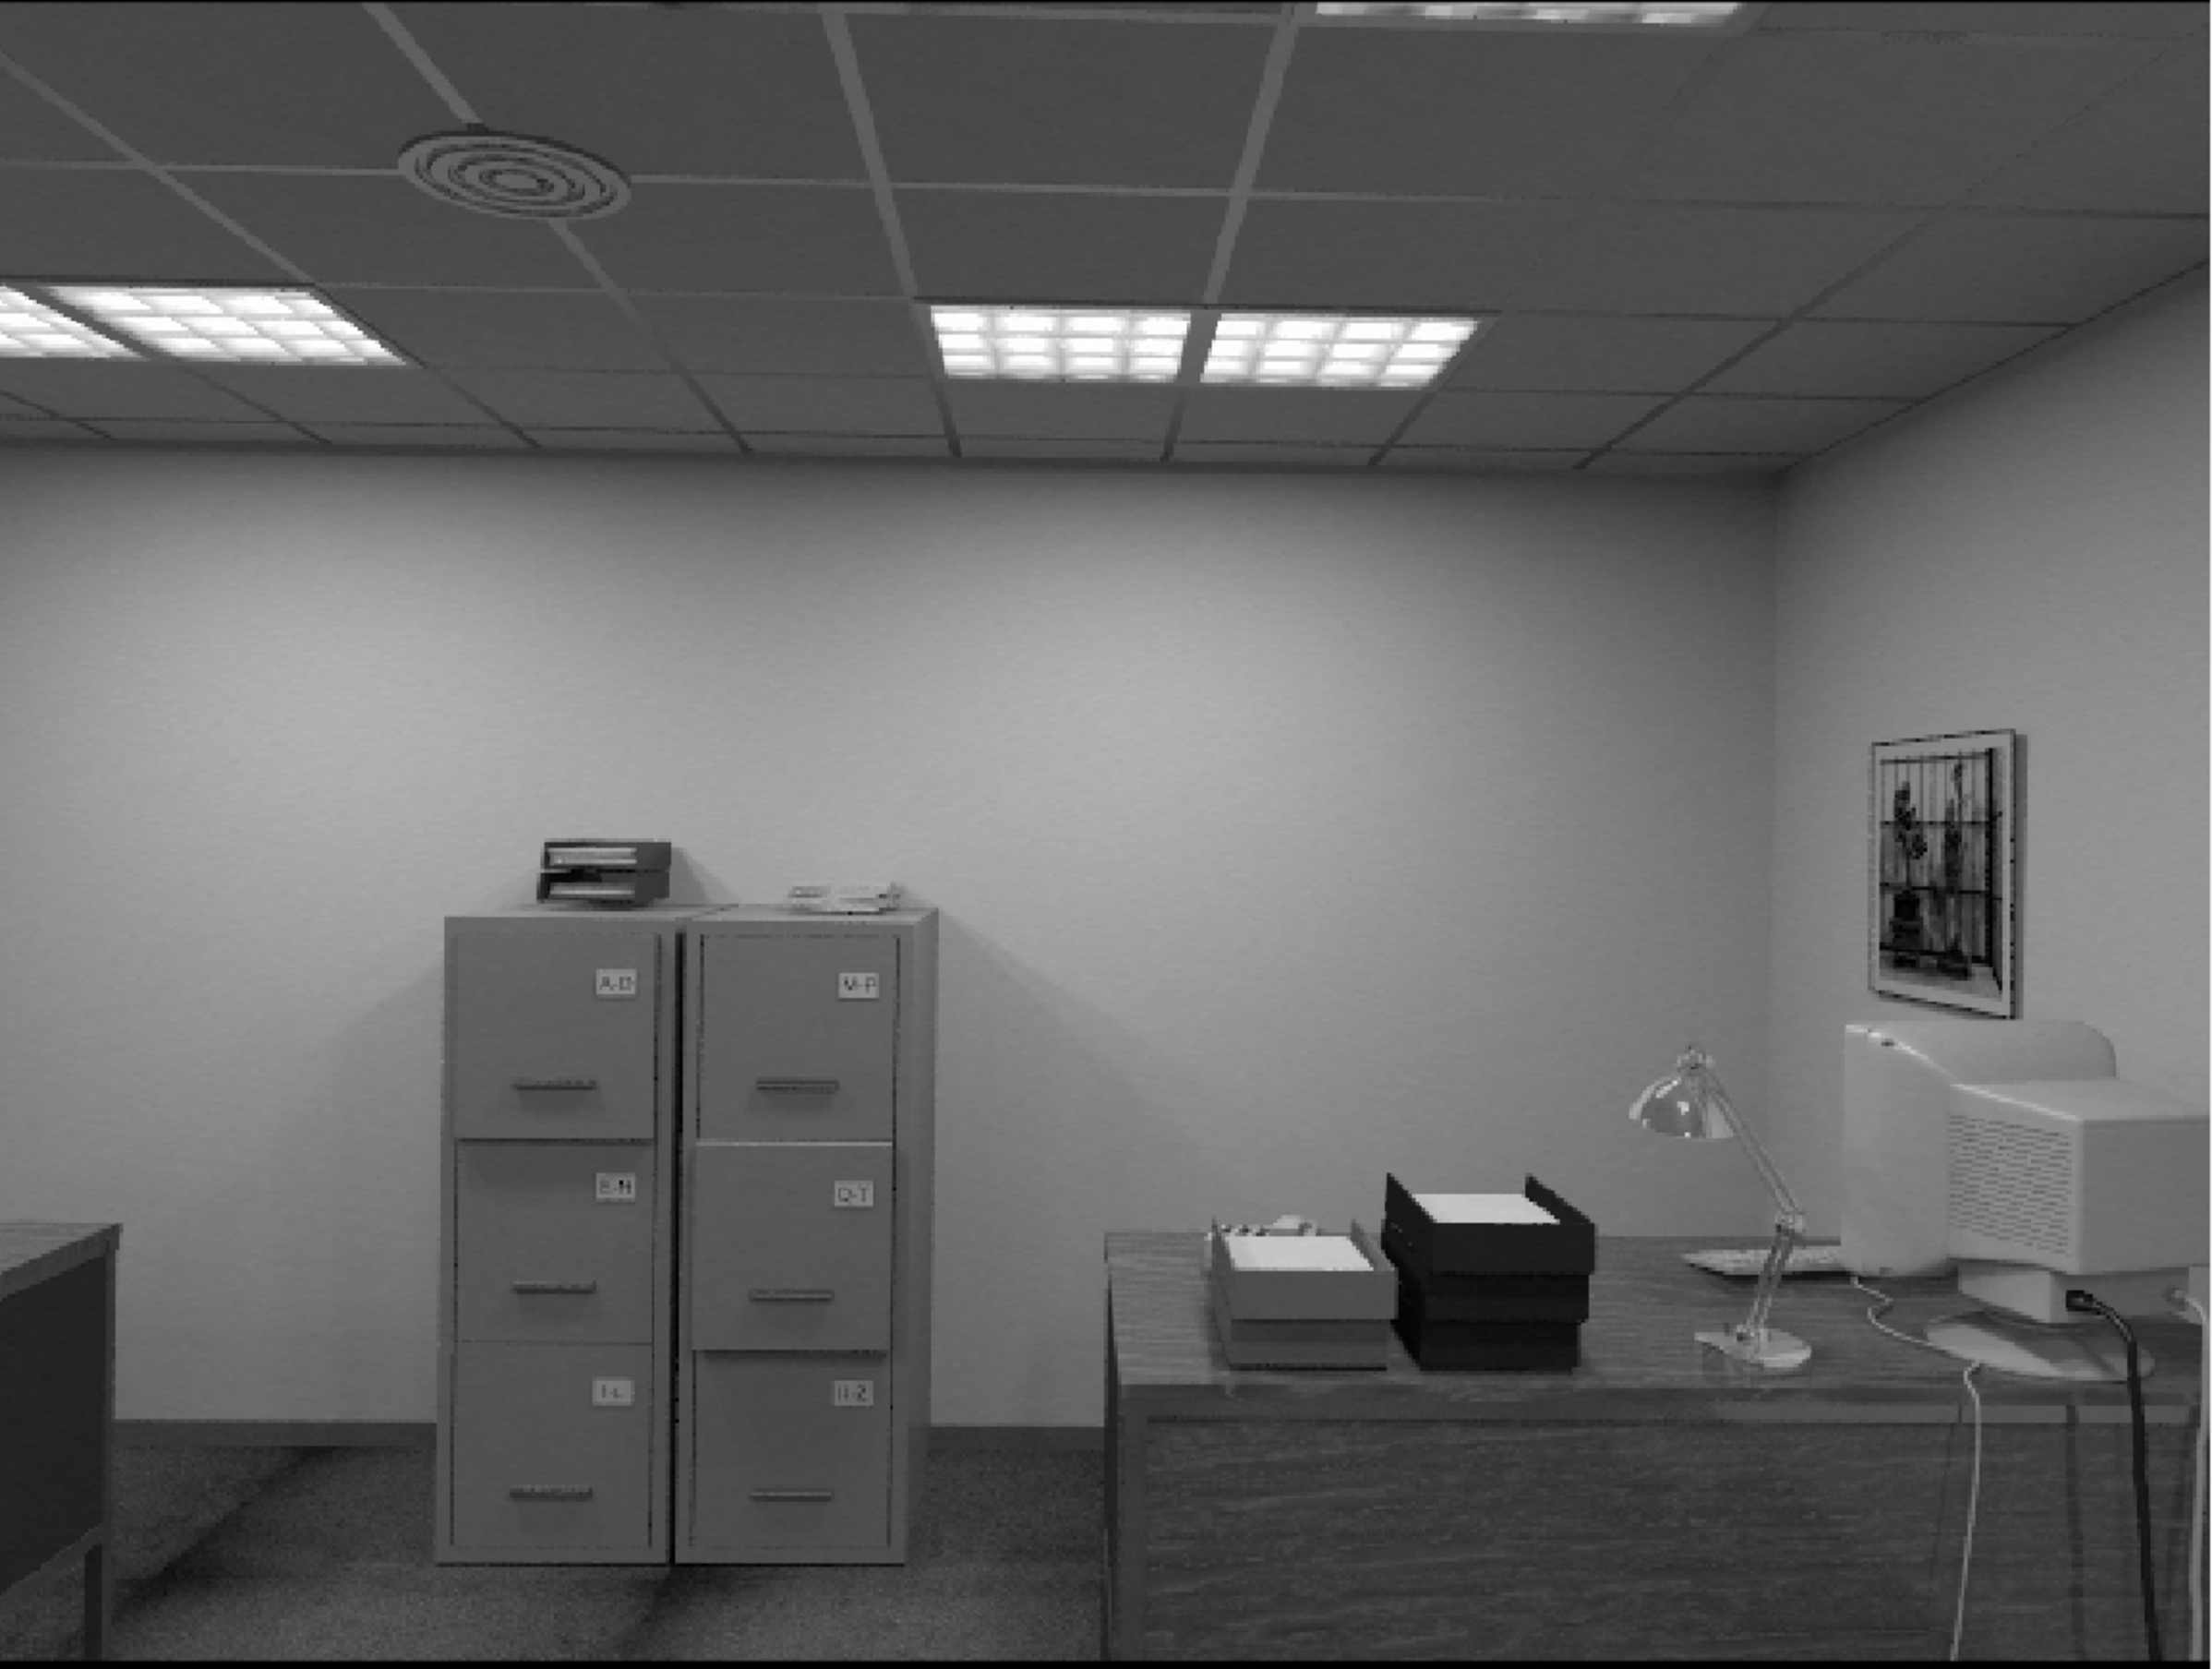
\includegraphics[height=1in]{of03.pdf}}
\caption{Characteristic images of selected typical sequences.} \label{fig:exampleimages}
\end{figure*}

\begin{figure}[th!]
  \centering
  \subfloat[Indoor + Outdoor\label{fig:dtree1_all}]
        {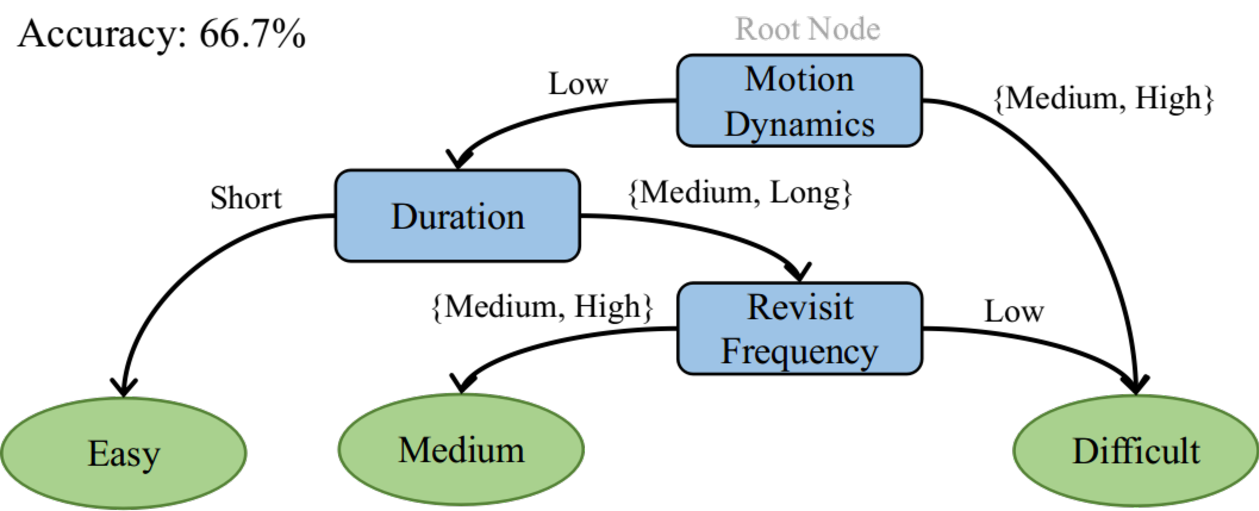
\includegraphics[width=0.80\columnwidth]{decision_tree_all.pdf}}
    \\
  \subfloat[Indoor Only\label{fig:dtree1_indoor}]
        {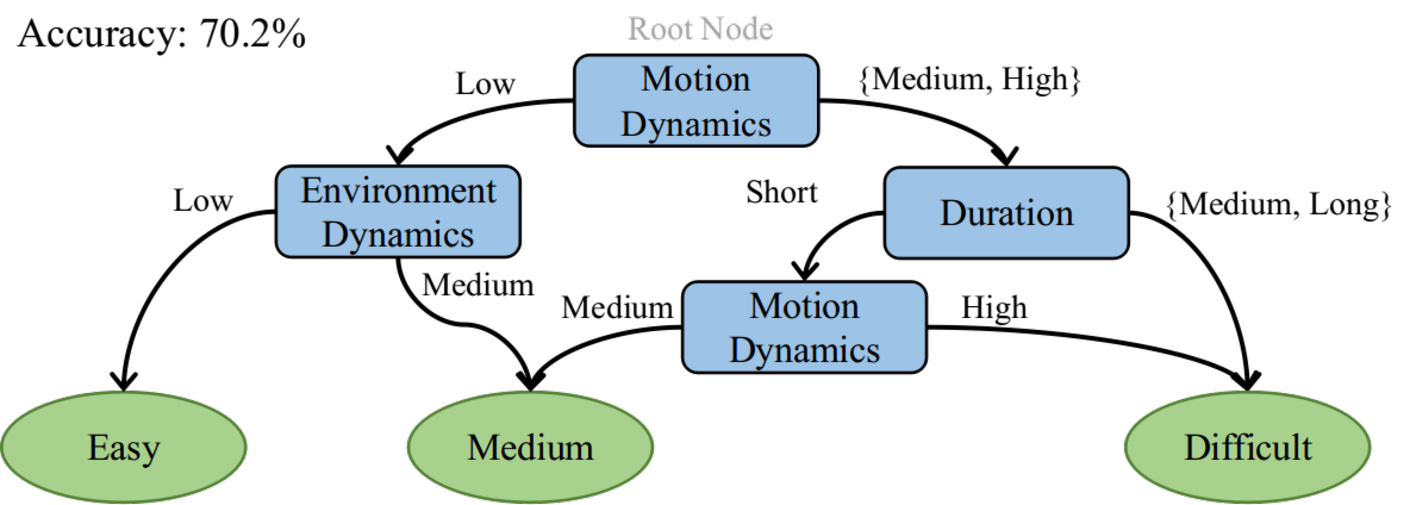
\includegraphics[width=0.80\columnwidth]{decision_tree_indoor.pdf}}
    \\
  \subfloat[Outdoor Only\label{fig:dtree1_outdoor}]
        {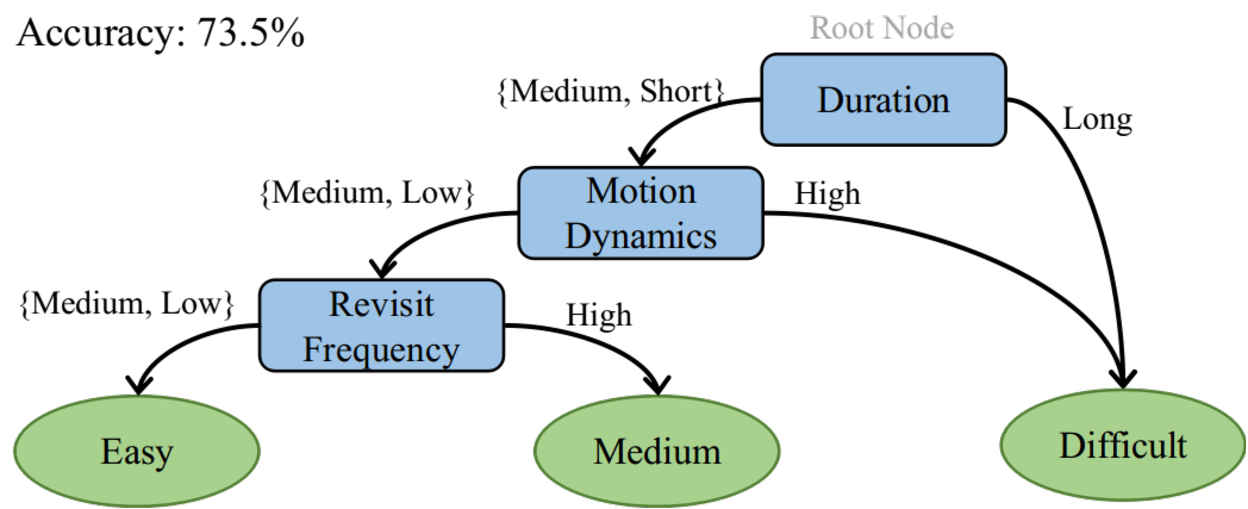
\includegraphics[width=0.80\columnwidth]{decision_tree_outdoor.pdf}}
  \caption{Trained Decision Tree Factors influencing difficulty level.} \label{fig:dtree1}
  \vspace*{-2em}
\end{figure}


As a first pass at understanding what factors most impact the difficulty
annotation, we applied a decision tree classifier to the annotated set of
chosen benchmarks.  Each sequence is an observation with the 
five
 properties as the predictors and \textit{Difficulty}
as the response. 
Cross-validation is adopted in the process to examine the predictive
accuracy of the fitted models and meanwhile to protest against overfitting.
Specifically, the training pool is partitioned into five disjoint subsets,
and the training process is performed on each subset to fit a model, which
is trained using four other subsets and validated using its own subset.
The best model is adopted and re-assessed using the whole training 
pool to report an accuracy.
Performing the training procedure for the entire benchmark set, the
indoor-only subset and the outdoor-only subset leads to three decision
trees, all depicted in Fig~\ref{fig:dtree1} with prediction accuracy noted 
above and to the left of each tree. 

Common factors for all of the trees are \textit{Motion Dynamics} and
\textit{Duration}, with \textit{Motion Dynamics} being fairly consistent
regarding the final outcome. \textit{Duration} is also consistent across
the trees, however \textit{medium} durations evaluate differently between
indoor and outdoor datasets.
For indoor sequences \textit{Environment Dynamics} plays a role in
differentiating \textit{easy} versus \textit{medium}, whereas for outdoor
sequences it does not. It may reflect the different sensor hardware
associated to the two use cases (wide vs narrow field-of-view) and the
relative size of the moving objects within the image stream.
Interestingly the \textit{Revisit Frequency} has an opposing outcome for the
full dataset versus the outdoor dataset, suggesting the opposite role
of this factor for the indoor dataset though it is not a dominant one.
Revisiting for outdoor scenes may reflect the nature of loop closure at
intersections. There are four ways to cross an intersection but only one
crossing direction can trigger or contribute to loop-closure. For indoor
scenes with more freedom of movement, there may actually be less diversity
in view direction during revists.



Based on the decision trees, challenging sequences should be those with high
motion dynamics or long duration (irrespective of the motion dynamics).
To generate a reference set of sequences spanning these different decision
variables and reflecting distinct pathways, we reviewed the dominant
factors and identified 12 characteristic sequences across the three
performance categories.  
The \textit{easy} sequences are \textit{Seq 04}, 
\textit{lr kt0}, 
\textit{f2 desk person};
the \textit{medium} sequences are 
\textit{Conf. Hall1}, 
\textit{Seq 02}, 
\textit{room3}, \textit{of kt3}; and the
\textit{difficult} sequences are \textit{MH 05 diff}, \textit{V1 03 diff}, 
\textit{Corridor}, \textit{NewCollege}, \textit{outdoors4}.
